%!TEX root = ../dissertation.tex

\section*{Thesis overview}

%!TEX root = ../dissertation.tex

\textbf{Relevance.}
Finite-state machines are one of the fundamental concepts in discrete mathematics, informatics, and software engineering.
Besides a direct role in the formal languages theory and design of computing devices, various finite-state machine models are practically used nowadays for
development and analysis of software.

For example, finite-state machines are used for development of software models for controllers and mission-critical systems\cite{shalyto-automata-2010-en,DBLP:conf/setta/PatilDV15},
protocol specification~\cite{DBLP:conf/coordination/JongmansHA14}, behavior modeling for complex high-level systems~\cite{DBLP:journals/ese/HeuleV13,wagner2006modeling}.
The main advantages of using finite-state machines include their relative simplicity for human perception and the possibility of automated formal verification of model properties~(model checking)~\cite{clarke2018model}.

In many cases the finite-state model is created by a developer manually, an example is the automata-based programming paradigm~\cite{shalyto-automata-2010-en}.
Other applications assume automated inference of a finite-state machine: extraction of the model from existing data or systems.
Among practical examples of finite-state model inference applications are:
synthesis of software models for controllers from manually or automatically collected behavior examples~\cite{DBLP:conf/etfa/ChivilikhinBUSS18}, 
synthesis of formal models for plants in control systems~\cite{DBLP:conf/etfa/BuzhinskyV17,DBLP:journals/tii/BuzhinskyV17}, 
analysis of interaction models for complex software systems~\cite{DBLP:journals/tosem/CookW98,DBLP:conf/sigsoft/BertolinoIPT09,DBLP:journals/ese/HeuleV13}  and network protocols~\cite{DBLP:conf/sp/SivakornAPKJ17}, etc.
Active research and development in finite-state machine inference algorithms began in the 1970's.
In 1978 Gold proved that the problem of inferring a deterministic finite automaton~(DFA) with the minimal number of states from given behavior examples is NP-complete~\cite{DBLP:journals/iandc/Gold78}.
This theoretical result emphasizes the complexity of the finite-state machine inference problem in the general case, actualizing the development of practically applicable algorithms.

Since then, a large variety of both heuristic and metaheuristic algorithms for finite-state machine inference from behavior examples have been proposed,
now comprising a whole class of algorithms in discrete mathematics.
In recent years a group of methods have been developed that are based on reductions of the problem of finding a minimal (in terms of the number of states) finite-state machine to other NP-complete problems.
The most efficient approaches are based on reductions to the Boolean satisfiability problem.

The Boolean satisfiability problem (SAT) consists of determining whether a satisfying assignment exists for a given Boolean formula.
According to the Cook-Levin theorem from 1971, the Boolean satisfiability problem is NP-complete.
This fact stimulated and actualized the development of practically applicable software tools for solving SAT.

SAT solving methods have been developed even before any theoretical complexity bounds were introduced.
In 1962 the Davis-Putnam-Logemann-Loveland~(DPLL)~\cite{DBLP:journals/cacm/DavisLL62} algorithm has been proposed for solving SAT: it is a complete algorithm with the capability of returning a 
satisfying assignment for satisfiable formulas, which is based the unit propagation rule and elimination of clean variables for accelerating the search.
This algorithm heuristically searches the space of all variable assignments and stops if a satisfying assignment has been found; if the algorithm completed the search and did not find a satisfying assignment, the formula is concluded to be unsatisfiable.

In the 1990's the Conflict Driven Clause Learning~(CDCL)~\cite{DBLP:conf/iccad/SilvaS96} algorithm has been proposed based on the DPLL algorithm: CDCL saves clauses derived from analyzing conflicts 
encountered in DPLL.
Such clauses allow the algorithm to much earlier decide the unsatisfiability of the formula with current assumptions, and switch to considering new assumptions.

The CDCL algorithm is the base of all modern software tools for solving SAT (SAT solvers).
Unlike the situation for all other NP-hard problems, the research community annually holds SAT solver competitions~\cite{sat-competitions,sat-competition-2020}.
This fact actualizes development of problem solving methods based on reductions to SAT:
to increase the efficiency of the method one does not need to change its source code, it will be sufficient to simply change the SAT solver to a more modern one.

However, in the methodology of reducing a given problem to SAT the fundamental question is not the used SAT solver, but the way an instance of the problem is translated to a Boolean formula,
for which a satisfying assignment will be searched.
For example, in recent years for the problem of inferring a minimal DFA from given behavior examples a basic reduction to SAT~\cite{heule-icgi10} and several of 
its extensions~\cite{DBLP:journals/ese/HeuleV13,ulyantsev-phd-13-en} have been developed.
The modifications proposed the use of symmetry-breaking predicates: auxiliary clauses that define a problem-dependent way of search space reduction.

These search space reduction techniques proved to be very effective in practice, allowing inference of finite-state machines of larger size than it was possible before.
However, consequent analysis shows that these techniques are not optimal, and the area of applicability of state-of-the-art methods for exact DFA synthesis from behavior examples is still quite limited
(which is, first of all, explained by the NP-completeness of the problem).
Thus, the topic of this thesis, which continues the described research of recent years and aims to extend the capabilities of methods for search space reduction and DFA inference, 
is \textbf{relevant} to this research domain.

\textbf{State of the art.}
The problem of inferring a deterministic finite automaton from behavior examples given by two sets $S_{+}$ and $S_{-}$ consists in finding a DFA with the minimal number of states,
such that all strings from the set $S_{+}$ are accepted by the automaton, and all strings from $S_{-}$ are rejected.
This problem was first formulated in Gold's paper in 1967~\cite{DBLP:journals/iandc/Gold67}.

The first known algorithm for solving this problem has been proposed in the work by Trakhtenbrot and Barzdin in 1970~\cite{trakhtenbrot-1973-modeling-en}: the \texttt{TB}-algorithm.
However, this algorithm only covers one special case of the problem of DFA inference from behavior examples:
sets $S_{+}$ and $S_{-}$ must contain all words of length $k$ over the alphabet $\Sigma$ (a total of $\abs{\Sigma}^{k}$ words).
In this algorithm, as in the majority of the following ones, behavior examples are represented as an augmented prefix tree: a prefix tree, in which vertices can be accepting, rejecting, or intermediate.
The \texttt{TB}-algorithm performs brute-force search of all possible pairs of states of the prefix tree, and merges equivalent states.

In 1978 Gold proved that the problem of finding a DFA of a given size (and thus of minimal size too) is NP-complete~\cite{DBLP:journals/iandc/Gold78}.
Due to this complexity result, development of new minimal DFA inference algorithm seized for a decade.
In the following years researchers started developing inexact heuristic algorithms, which do not guarantee the minimality of the found DFA.
Among these algorithms are: \texttt{traxbar}~\cite{DBLP:conf/colt/Lang92}, \texttt{RPNI}~\cite{oncina-rpni-1992}, \texttt{EDSM}~\cite{DBLP:conf/icgi/LangPP98}, \texttt{exbar}~\cite{lang-1999-faster}, \texttt{Windowed-EDSM}~\cite{DBLP:conf/icgi/CicchelloK02}.
All mentioned algorithms are based on merging the states of the augmented prefix tree.
The states for merging are selected heuristically: this explains the high efficiency of these algorithms and their inexactness.

Another common approach to DFA inference from behavior examples is the application of metaheuristic algorithms.
For example, evolutionary~\cite{DBLP:journals/pami/LucasR05,DBLP:conf/cec/Gomez06} and ant colony optimization~\cite{chivilikhin-12-ant} algorithms have been proposed.
Metaheuristic algorithms are also inexact: they do not even guarantee that any solution will be found in finite time.

Scientists from Netherlands Heule and Verwer proposed in 2010 an algorithm \texttt{DFASAT} that can infer a DFA of guaranteed minimal size from arbitrary behavior examples~\cite{heule-icgi10}.
The algorithm is based on a reduction of the problem of DFA inference from behavior examples to SAT, where an arbitrary step is a reduction to graph coloring proposed in 1997~\cite{Coste97regularinference}.
For reducing the size of the search space during SAT solving Heule and Verwer proposed a number of symmetry breaking approaches: consistency graph, auxiliary clauses, search for a large clique.
However, even with all these techniques, in reasonable time \texttt{DFASAT} can infer automata with no more than ten states.
In order to simplify the problem, Heule and Verwer proposed to use the \texttt{EDSM} algorithm to make several merges in the augmented prefix tree prior to using the SAT approach: however, this leads to the whole algorithm becoming inexact, and the DFA minimality guarantee is lost.

Later, the author of the thesis together with his supervisor Vladimir Ulyantsev and professor Anatoly Shalyto proposed symmetry breaking predicates based on the breadth-first search algorithm
(BFS)~\cite{zakirzyanov2015LATA}.
For each DFA with $M$ states there exist $\mathcal{O}\left(M!\right)$ isomorphic automata, which are distinct from the point of view of a SAT solver.
The proposed symmetry breaking predicates yield a considerable reduction of the search space during SAT solving: instead of a factorial of isomorphic automata, only one representative of each
isomorphism equivalence class is considered during search.
This one representative is a DFA with states enumerated in the order of BFS traversal.
This method is the most efficient among known methods for exact DFA inference from behavior examples, and allows inference of automata with up to 40 states.
However, analysis showed that the proposed na\"ive SAT encoding of BFS predicates is not optimal: the resulting Boolean formula is too large.
Furthermore, symmetry breaking predicates based on depth-first search~(DFS) have not been considered.

Among other drawbacks of SAT-based DFA inference methods an important one is the dependence of the size of the Boolean formula from the size of the behavior examples.
Sets of behavior examples are often excessive and contain unnecessary words.
Literature analysis showed that no intellectual methods of choosing a subset of behavior examples have been proposed earlier.
A possible solution is the application of \emph{counterexample-guided abstraction refinement}~(CEGAR)~-- an iterative algorithm initially proposed for software model inference~\cite{DBLP:conf/cav/ClarkeGJLV00,мандрыкин2013введение-en}.

The opposite situation is inference of a DFA from small sets of behavior examples.
In this case it may be beneficial to infer all corresponding minimal non-isomorphic DFA for further analysis.
Also, the existence of a single unique DFA of minimal size for a given set of training data illustrates the quality of the latter.
However, the problem of inferring all non-isomorphic DFA has not been considered before by the research community, and thus no efficient methods have been proposed.

The \textbf{aim} of this thesis is to increase the efficiency of exact methods for deterministic finite automata inference from given behavior examples by means of reducing the search space during Boolean satisfiability problem solving.
In order to achieve this aim, the following \textbf{tasks} have been defined and completed:
\begin{enumerate}
  \item Development of symmetry breaking predicates based on SAT encodings of the breadth-first and depth-first graph search algorithms for reducing the search space during SAT solving.
  Development and implementation of exact methods for DFA inference from behavior examples using said predicates, and experimental evaluation of developed methods.

  \item Development and implementation of an exact method for DFA inference from an excessive set of behavior examples using a reduction to SAT and counterexample-guided abstraction refinement.
  Experimental evaluation of the developed method.
  
  \item Development and implementation of a method for inferring all non-isomorphic DFA of minimal size from given behavior examples using symmetry breaking predicates and SAT solvers.
  Experimental evaluation of the developed method.
\end{enumerate}

The \textbf{object of the study} is the problem of DFA inference from given behavior examples.

The \textbf{subject of the study} are exact DFA inference methods that use Boolean satisfiability solvers.

\textbf{Compliance with specialty requirements.} The thesis complies with \S 10 
``Development of foundations of mathematical theory of formal languages and grammars, finite automata theory, and graph theory''.

\textbf{Principal statements of the thesis:}
\begin{enumerate}
  \item An \emph{approach} for constructing symmetry breaking predicates based on SAT encodings of breadth-first and depth-first graph search algorithms for the purpose of reducing the search space during SAT solving.
  Exact \emph{methods} for DFA inference from given behavior examples that use the said predicates.
  
  \item An exact \emph{method} for DFA inference from an excessive set of behavior examples using a reduction to SAT and counterexample-guided abstraction refinement.
  
  \item A \emph{method} for inferring all non-isomorphic DFA of minimal size from given behavior examples using symmetry breaking predicates and SAT solvers.
\end{enumerate}

The \textbf{scientific novelty} of the thesis is as follows:
\begin{enumerate}
  \item Symmetry breaking predicates based on a SAT encoding of the depth-first search algorithm have not been proposed before.
  The proposed symmetry breaking predicates based on the breadth-first search algorithm are expressed with a Boolean formula that is comprised of an asymptotically smaller number of clauses in comparison to the existing approach. 
  Moreover, new symmetry breaking predicates that utilize special features of the breath-first search tree are proposed.

  \item Previously, no exact DFA inference methods for the case of an excessively large number of behavior examples have been proposed.
  The use of counterexample-guided abstraction refinement together with a reduction to SAT allows for DFA inference from an excessive set of behavior examples through
  iteratively adding only meaningful examples until a DFA satisfying the whole excessive set will be inferred.

  \item No methods for inferring all non-isomoprhic DFA of minimal (or any fixed) size satisfying given behavior examples have been previously proposed.
\end{enumerate}

\textbf{Research methodology and methods.} 
The methodological basis of the thesis is formed by the principles of formalization, generalization, deductive and inductive substantiation of statements, experimental evaluation and analysis of experimental results.
This thesis uses methods of automata theory, graph theory, probability theory, discrete mathematics, object oriented programming, experiment design and analysis.

\textbf{Soundness and correctness} of scientific results obtained in this thesis is confirmed by correct justification of problem settings, precise formulation of criteria,
as well as by the results of experimental evaluation of the proposed methods.

The \textbf{theoretical significance} of the thesis is that it proposes new methods for search space reduction during SAT solving for the problem of DFA inference, namely, symmetry breaking predicates based on SAT encodings of breadth-first and depth-first graph search algorithms:
\begin{itemize}
  \item a SAT encoding of the DFS-enumeration property of a DFA is proposed;
  \item a new SAT encoding of the BFS-enumeration property of a DFA is proposed that requires an asymptotically smaller number of clauses than before;
  \item a SAT encoding of various properties of the BFS traversal tree is proposed.
\end{itemize}
Furthermore, the thesis proposes an approach that combines a SAT-based DFA inference method with counterexample-guided abstraction refinement.
Also, the developed symmetry breaking predicates enable the proposal of a method for the problem of inferring all non-isomorphic DFA of minimal size, which previously did not have efficient solving methods.

The \textbf{practical significance} of the thesis lies in efficiency improvement of exact methods for DFA inference from given behavior examples.
Experiments showed that the proposed method for DFA inference from given behavior examples using BFS-based symmetry breaking methods
is the most efficient one among known exact methods and allows inferring automata of larger size than previously proposed methods.
The developed exact method for DFA inference from an excessive set of behavior examples using a SAT encoding and CEGAR allows efficient inference of automata in 
the case when the size of the behavior examples is too large, and the resulting Boolean formula is too large to process for modern SAT solvers.
The developed method of inferring all non-isomorphic DFA of minimal size from given behavior examples using symmetry breaking predicates and SAT solvers is the first known
method for inferring all non-isomorphic automata.
It also allows one to estimate the completeness of the data represented by behavior examples by means of proving the existence or absence of a single minimal-sized DFA that describes the data.

Moreover, all developed methods and approaches may later be adapted for application to inference of more complex finite-state models~\cite{ulyantsev-phd-13-en}.
For example, the proposed method for inferring all non-isomorphic DFA has been adapted to synthesize state machines that model the behavior of programmable logic controllers~\cite{DBLP:journals/tii/ChivilikhinPCCV20}.

The results of the thesis \textbf{were used} in the project SAUNA (``Integrated safety assessment and justification of nuclear power plant automaton'') by the ``IT in Industrial Automation'' research group of the department of electrical engineering and automation in Aalto University, Finland, in the framework of the Finnish research program in 
safety of nuclear power plants SAFIR2018\footnote{http://safir2018.vtt.fi/}.
In particular, one of the project tasks was to develop a model inference method for various control systems of nuclear power plants components from given behavior examples and linear temporal logic specification.
This task was solved using counterexample-guided abstraction refinement in a similar way to the one proposed by the author of the thesis for DFA inference.
This is confirmed by a letter from the principal investigator of the ``IT in Industrial Automation'' group, Valeriy Vyatkin.

Results of this thesis have also been used in the project No.~18-37-00425 ``Development of efficient machine learning methods for deterministic finite automata inference
based on Boolean satisfiability solving'' (2018--2020) funded by the Russian Foundation for Basic Research and led by the author of the thesis.

Results have also been used in the framework of the governmental financial support of leading universities in Russia, grant 074-U01 (project ``Bioinformatics, machine learning, programming technologies, coding theory, proactive systems'', 2013--2017) and grant 08-08 (project ``Methods, models and technologies of artificial intelligence in 
bioinformatics, social media, cyber-physical, biometric and speech systems'', 2018--2020).

Results are also used in the ``Design of automata-based programs'' course of the ``Mathematical models and algorithms in software engineering'' Bachelor's program of the 
Faculty of Information Technologies and Programming (supported by the official act of use).

\textbf{Dissemination.}
The main results of the thesis were presented at the following venues:
\begin{enumerate}
  \item 9\textsuperscript{th} International Conference on Language and Automata Theory and Applications (LATA 2015). 2015, Nice, France.
  \item 6\textsuperscript{th} International Symposium ``From Data to Models and Back (DataMod)''. 2017, Trento, Italy.
  \item 16\textsuperscript{th} IEEE International Conference on Industrial Informatics (INDIN 2018). 2018, Porto, Portugal.
  \item 13\textsuperscript{th} International Conference on Language and Automata Theory and Applications (LATA 2019). 2019, Saint Petersburg.
  \item IV-VII Russian Young scientists congress. 2015-2018, Saint Petersburg.
  \item IX Young scientists congress. 2020, Saint Petersburg.
  \item XLVI Scientific and educational-practical conference of ITMO University. 2017, Saint Petersburg.
  \item XLVIII Scientific and educational-practical conference of ITMO University. 2019, Saint Petersburg.
\end{enumerate}

\textbf{Personal contribution.}
The ideas of symmetry breaking predicates based on depth-first search, of the DFA inference method using these predicates, as well as implementation of an algorithm
based on the proposed method and its experimental evaluation belong to the author.
The idea of symmetry breaking predicates based on breadth-first search that require an asymptotically smaller number of clauses in the encoding, the idea of
SAT encoding of BFS tree properties, and the idea of the DFA inference method that uses these results belong to the author of the thesis and Jo{\~{a}}o Marques-Silva;
the implementation of algorithms based on proposed methods belong to the author, experimental evaluation belongs to the author and Alexey Ignatiev.
The idea of an exact method for DFA inference from behavior examples using a reduction to SAT and counterexample-guided abstraction refinement,
the implementation of an algorithm based on the proposed method and experimental evaluation belong to the author.
The idea of the exact method for inferring all minimal-sized DFA from given behavior examples using SAT solvers belongs to the author and the supervisor Vladimir Ulyantsev,
implementation of the algorithm based on the proposed method and experimental evaluation belongs to the author.
In papers co-authored with the supervisor, Vladimir Ulyantsev, his contribution consists of the general supervision of the work.

\textbf{Publications.}
The main results of this thesis are presented in ten publications, four of which are indexed in Scopus, and one is published in a journal included into the 
List of the Higher Attestation Commission.
Also the author has one publication indexed in Scopus on another topic from the machine learning domain.

\section*{Thesis contents}

The \textbf{introduction} of the thesis contains the relevance of the research, a formulation of the aim, objectives, principal statements of the thesis, as well as scientific novelty, theoretical and practical significance of the work.

\textbf{\underline{Chapter 1}} presents an analytical review of the research domain and existing research results in the area of deterministic finite automata inference.
It also introduces the terminology, main definitions and known results from a number of topics in informatics that are necessary for the description of methods and algorithms proposed in the thesis.

\insectionen{\ref{sec:review:sat}} a formal setting of the Boolean satisfiability problem is given along with necessary definitions and
a brief description of the main approaches for solving this problem.
Also this section describes an approach to solving NP-hard problems through their polynomial-time reduction to the Boolean satisfiability problem.
Moreover, a brief overview of existing software tools for solving the Boolean satisfiability problem (SAT solvers) is given.

A Boolean formula is in \emph{conjunctive normal form} (CNF) if it is a conjunction of clauses, where each clause is a disjunction 
of literals.
The \emph{Boolean satisfiability problem} (\emph{satisfiability problem}, SAT) consists of determining, whether for a given Boolean formula in CNF there exists a satisfying assignment: a set of values of its variables for which the formula is true.
SAT is the historically first problem for which NP-completenss has been proved: any problem from NP can be reduced to SAT in polynomial time.
This fact explains the relevance of the development of more and more efficient SAT solvers.
The research community annually holds competitions to determine the best SAT solver; this fact also contributes to continuous development of this area.
The basis of all modern SAT solvers is the \emph{conflict driven clause learning}~(CDCL) strategy.

The approach to solving problems from NP, in which a reduction to SAT is devised and then a SAT solver is used to find a satisfying
assignment of the constructed Boolean formula, often turns out to be much more efficient and simpler than the development of a practically applicable method that directly solves the original problem.
Another important advantage of this approach is the fact that it is enough to write a reduction to the SAT once, and then, without applying any effort, use the progress of SAT solvers, choosing the most efficient one.



\insectionen{\ref{sec:review:dfa-inf}} basic concepts of deterministic finite automata and the formulation of the problem of inferring deterministic finite automata from behavior examples are given.
Behavior examples for some DFA $\mathcal{D}$ are defined as two sets of words $S_{+}$ and $S_{-}$ over the symbols of the DFA's alphabet, such that all words from $S_{+}$ belong the the language $\mathcal{L}\left(\mathcal{D}\right)$ and must be accepted by the DFA, and all words from $S_{-}$ do not belong to the language $\mathcal{L}\left(\mathcal{D}\right)$ 
and must be rejected by  the DFA.
The problem of DFA inference from behavior examples consists in finding a DFA of minimal size (with the minimal number of states) that
satisfies given behavior examples.
Previously it has been shown that this problem is NP-complete, as well as the problem of finding a DFA of any given size that satisfies given behavior examples.
An example of a DFA that satisfies behavior examples $S_{+} = \{aba, bb, bba\}$ and $S_{-} = \{b, ba\}$ is shown in Figure~\ref{syn-en:img:dfa-ex}.
One can notice that an automaton with two states satisfying sets $S_{+}$ and $S_{-}$ does not exist.
\begin{figure}[ht]
  \centering
  \ifafour
    \input{img/FIG1-a4}
    % 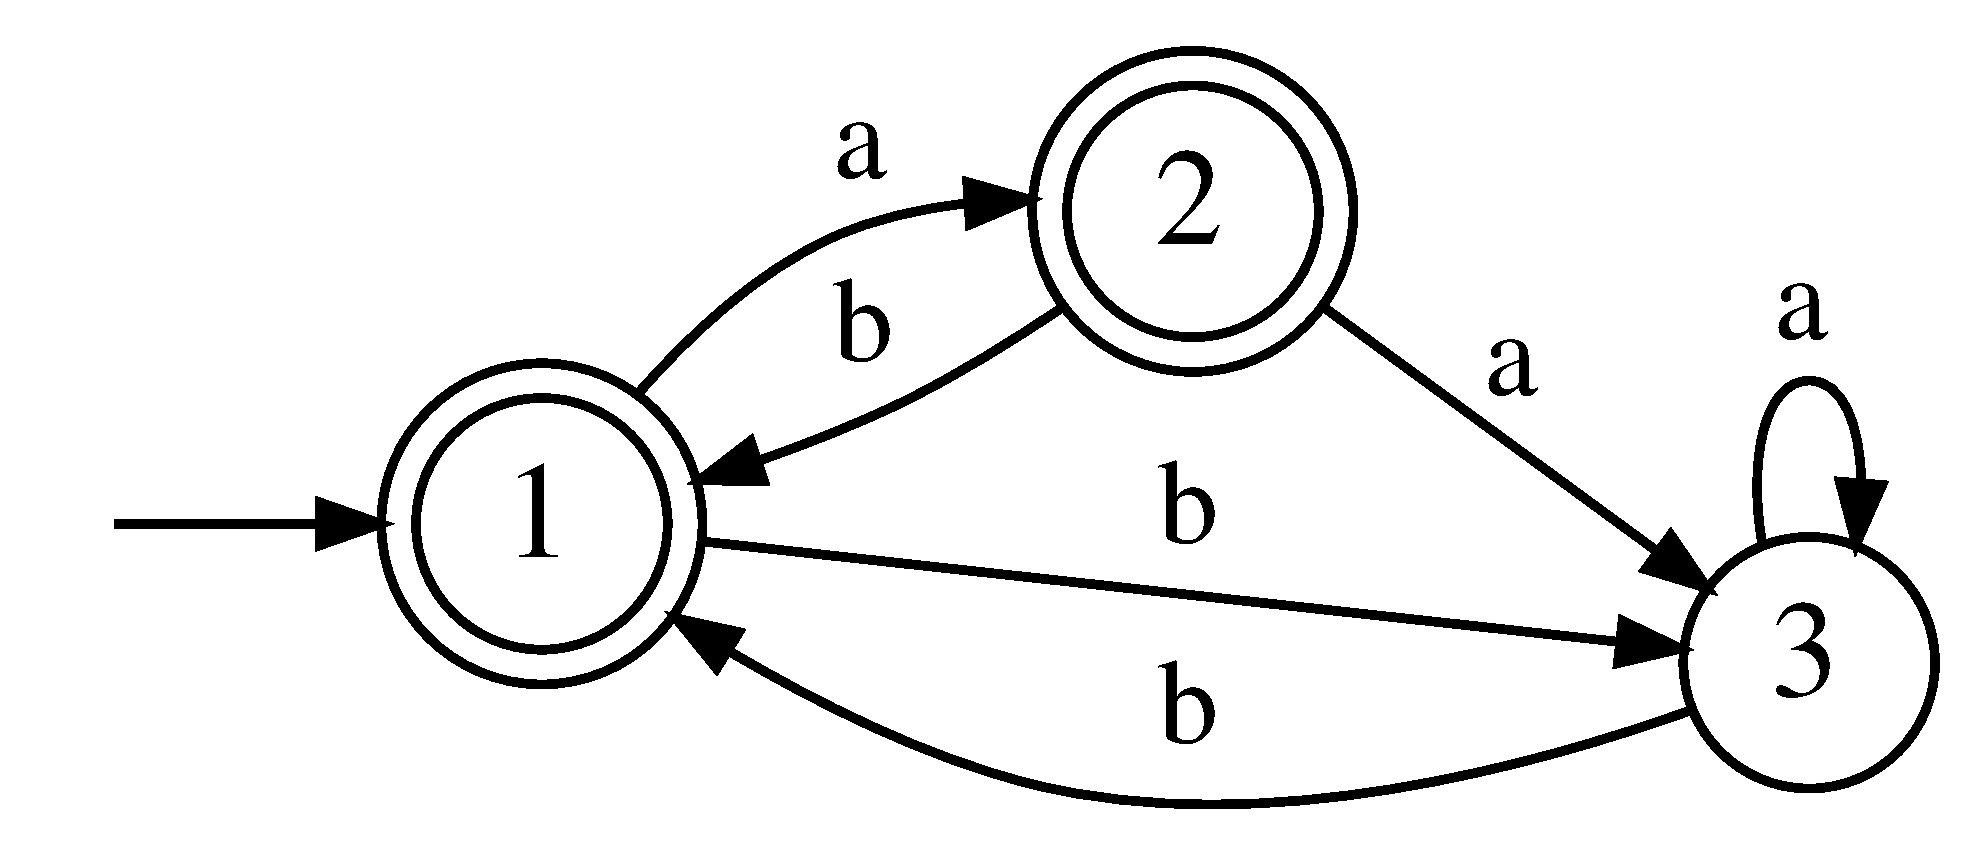
\includegraphics[scale=0.16]{img/datamod/FIG1.eps}
  \else
    \begin{tikzpicture}[
    ->, % makes the edges directed
    >=stealth', % makes the arrow heads bold
    node distance=1.9cm, % specifies the minimum distance between two nodes. Change if necessary.
    every state/.style={thick, fill=gray!10, minimum size = 0pt}, % sets the properties for each ’state’ node
    initial text=$ $, % sets the text that appears on the start arrow
]
    \node[state, initial, accepting] (q1) {$1$};
    \node[state, accepting] (q2) [above of=q1, xshift=1.9cm/2, yshift=-0.3cm] {$2$};
    \node[state] (q3) [right of=q1] {$3$};

    \path
        (q1) edge [bend right=10, below] node [xshift=2pt] {a} (q2)
        (q2) edge [bend right=10, above] node [xshift=-2pt] {b} (q1)
        (q1) edge [bend right=10, below] node {b} (q3)
        (q3) edge [bend right=10, above] node {b} (q1)
        (q2) edge [above] node [xshift=2pt] {a} (q3)
        (q3) edge [loop above] node {a} (q3)
        ;
\end{tikzpicture}
  \fi
  \caption{An example of a minimal DFA satisfying behavior examples $S_{+} = \{aba, bb, bba\}$ and $S_{-} = \{b, ba\}$}
  \label{syn-en:img:dfa-ex}
\end{figure}

\textbf{Section~\ref{sec:review:heuristic-dfa-inf}} presents an overview of existing heuristic and metaheurstic methods and algorithms
for DFA inference from behavior examples.
Heuristic algorithms include the \emph{evidence-driven state merging}~(EDSM) algorithm.
Metaheuristic algorithms include evolutionary strategies, genetic algorithms, and ant colony optimization algorithms.

Note that the mentioned approaches are inexact: they do not guarantee that the found DFA contains the minimal number of states, and, in some cases, they do not even guarantee that any DFA satisfying the behavior examples will be found.

\insectionen{\ref{sec:review:sat-dfa-inf}} an overview of existing methods for inferring DFA from behavior examples based on reduction to SAT is given. Unlike heuristic and metaheuristic approaches, these methods are exact: it is guaranteed that the automaton corresponding to the behavior examples will be found in finite time and will contain the minimum possible number of states.

The first step of considered methods is the construction of the \emph{augmented prefix tree acceptor}~(APTA): a tree-like data structure 
based on the ordinary prefix tree, in which each vertex is either not marked, or marked as accepting or rejecting.
An example of an augmented prefix tree is shown in~\ref{syn-en:img:apta-ex}.

\begin{figure}[ht]
  \centering
  \ifafour
    \begin{tikzpicture}[
    ->, % makes the edges directed
    >=stealth', % makes the arrow heads bold
    node distance=2cm, % specifies the minimum distance between two nodes. Change if necessary.
    every state/.style={thick, fill=gray!10, minimum size = 0pt}, % sets the properties for each ’state’ node
    initial text=$ $, % sets the text that appears on the start arrow
    double distance between line centers=2pt
]
    \def\yshift{0.47cm}
    \def\xshift{0.26cm}

    \node[state, initial] (q1) {$1$};
    \node[state, fill=white, dashed, inner sep=9.7pt] (q5) [above right of=q1, yshift=-\yshift, xshift=\xshift] {};
    \node[state, inner sep=4.2pt] (dummy5) [above right of=q1, yshift=-\yshift, xshift=\xshift] {$5$};
    \node[state, accepting] (q6) [right of=q5] {$6$};
    \node[state, accepting] (q7) [right of=q6] {$7$};
    \node[state] (q2) [below right of=q1, yshift=\yshift, xshift=\xshift] {$2$};
    \node[state] (q3) [right of=q2] {$3$};
    \node[state, accepting] (q4) [right of=q3] {$4$};
    \node[state, fill=white, dashed, inner sep=9.7pt] (q8) [above of=q6, yshift=-0.78cm] {};
    \node[state, inner sep=4.2pt] (dummy8) [above of=q6, yshift=-0.78cm] {$8$};

    \path 
        (q1) edge [above] node {b} (q5)
        (q5) edge [below] node {b} (q6)
        (q6) edge [below] node {a} (q7)
        (q5) edge [above] node {a} (q8)
        (q1) edge [below] node {a} (q2)
        (q2) edge [below] node {b} (q3)
        (q3) edge [below] node {a} (q4)
        ;
\end{tikzpicture}
    %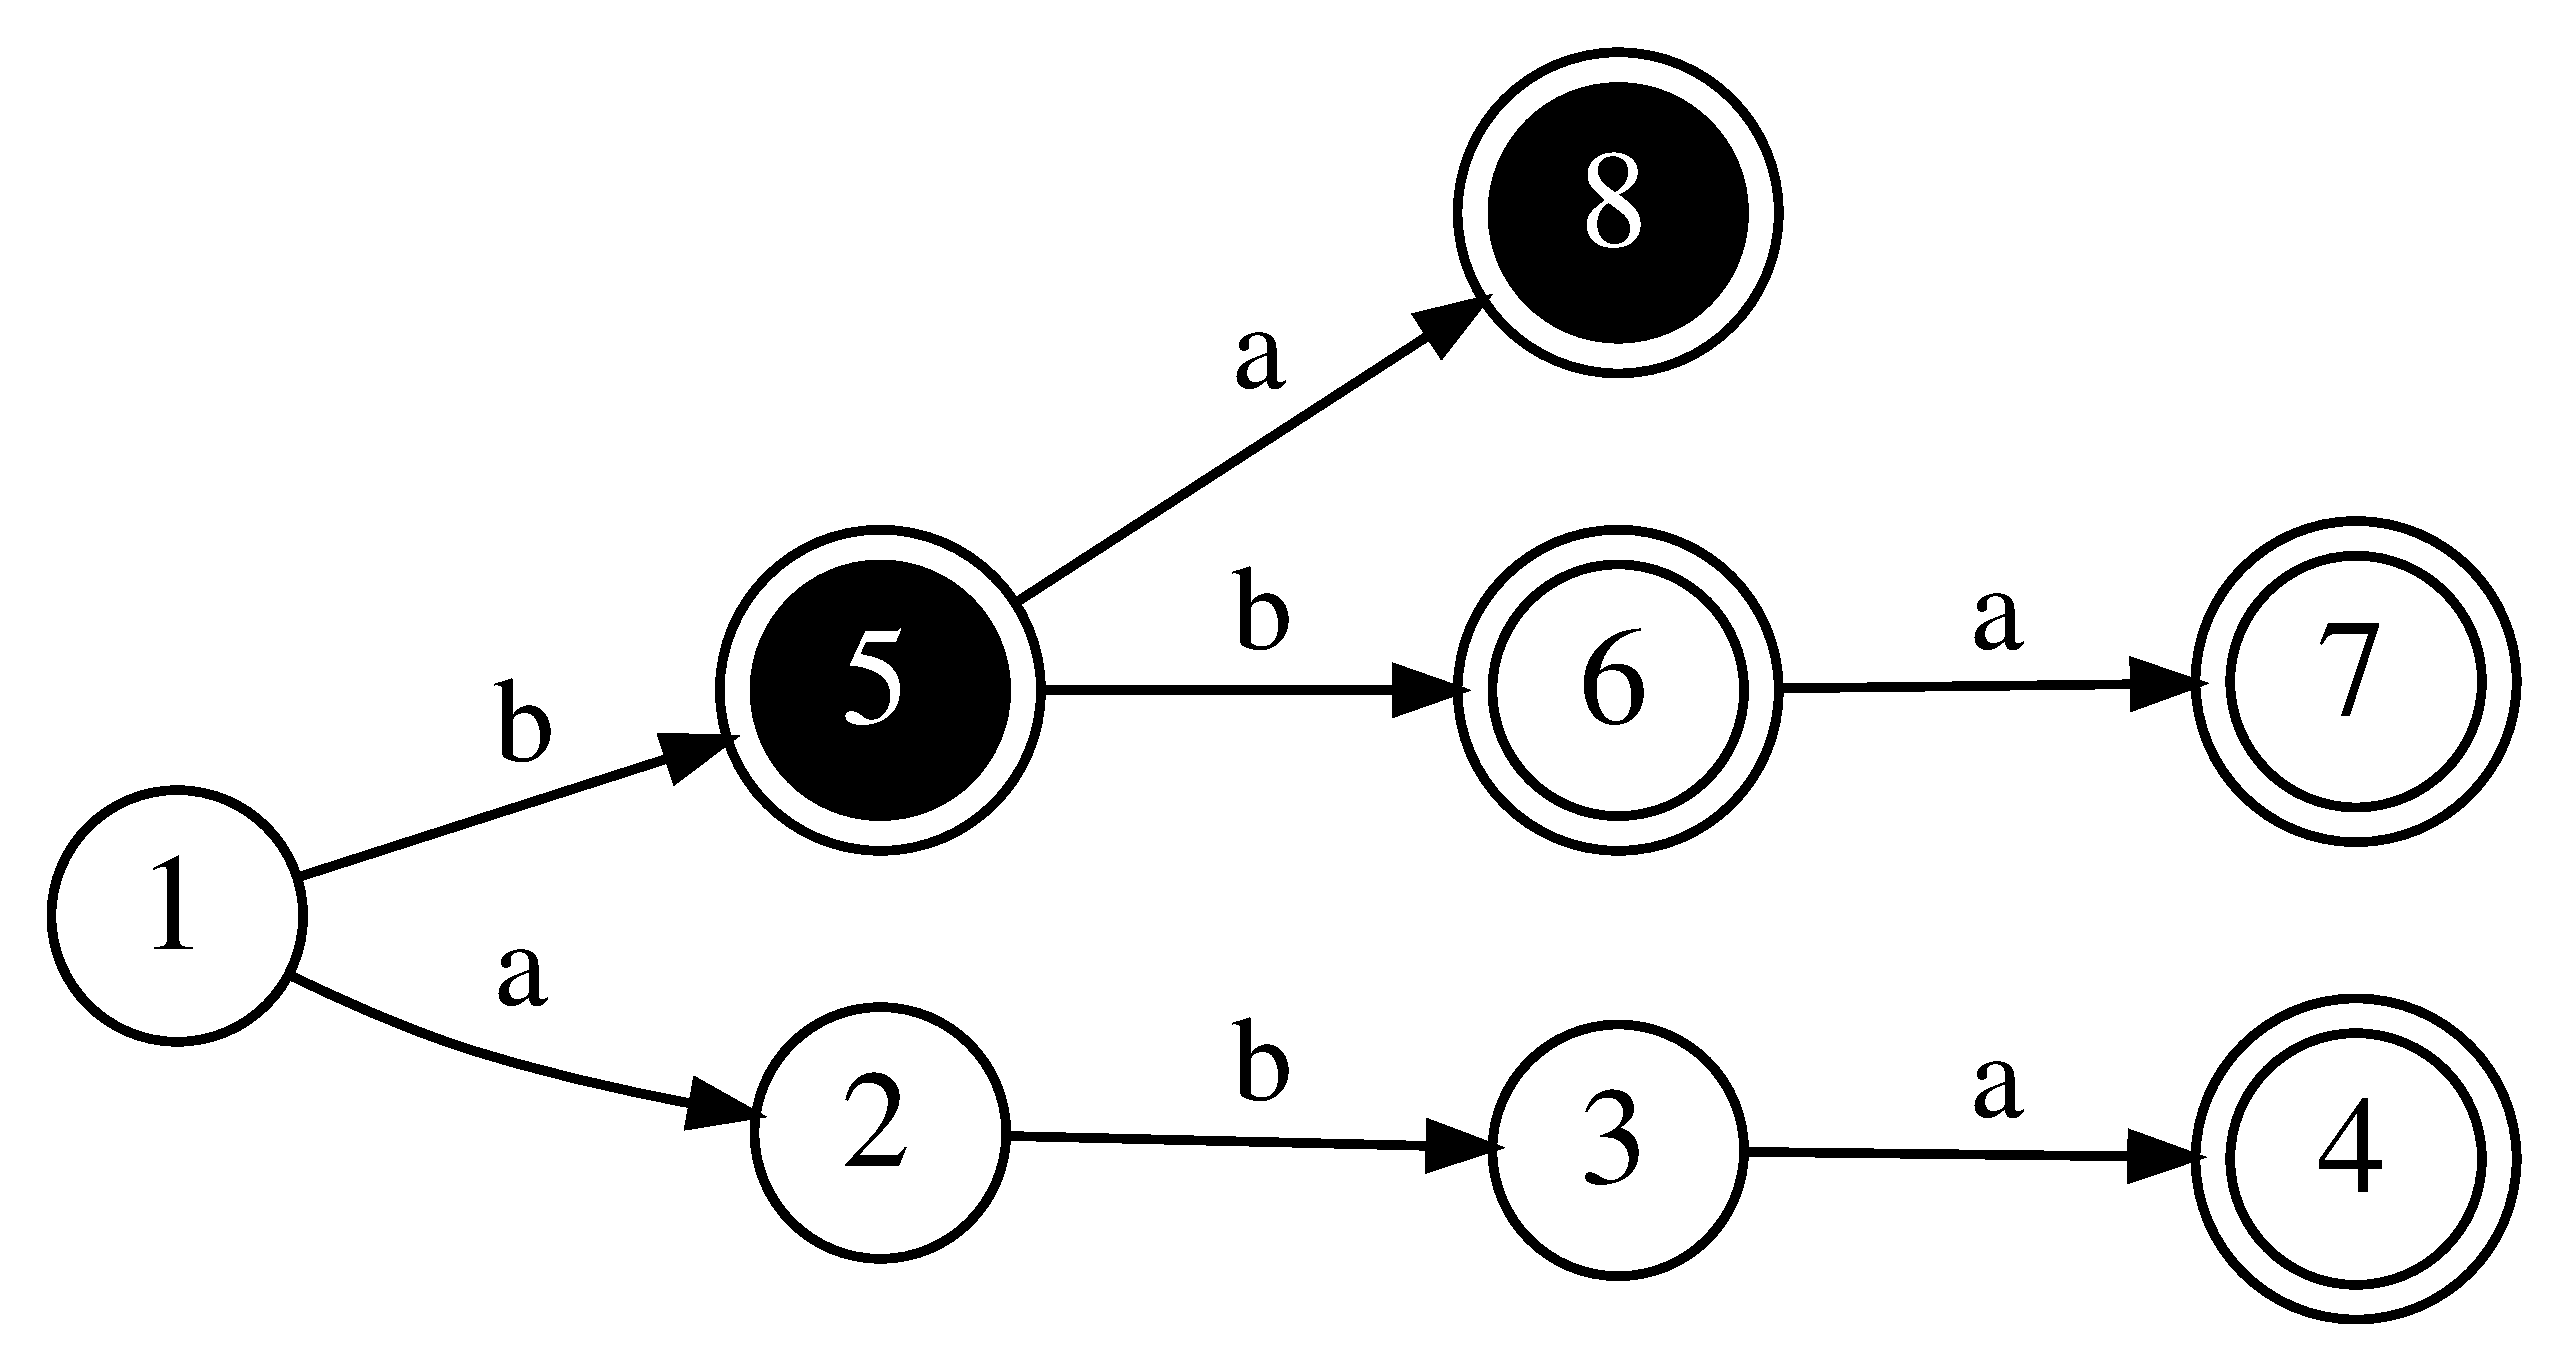
\includegraphics[scale=0.14]{img/datamod/FIG2a.eps}
  \else
    \begin{tikzpicture}[
    ->, % makes the edges directed
    >=stealth', % makes the arrow heads bold
    node distance=1.5cm, % specifies the minimum distance between two nodes. Change if necessary.
    every state/.style={thick, fill=gray!10, minimum size = 0pt}, % sets the properties for each ’state’ node
    initial text=$ $, % sets the text that appears on the start arrow
]
    \def\yshift{0.36cm}
    \def\xshift{0.2cm}

    \node[state, initial] (q1) {$1$};
    \node[state, dashed, inner sep=7pt] (q5) [above right of=q1, yshift=-\yshift, xshift=\xshift] {};
    \node[state, inner sep=3pt] (dummy5) [above right of=q1, yshift=-\yshift, xshift=\xshift] {$5$};
    \node[state, accepting] (q6) [right of=q5] {$6$};
    \node[state, accepting] (q7) [right of=q6] {$7$};
    \node[state] (q2) [below right of=q1, yshift=\yshift, xshift=\xshift] {$2$};
    \node[state] (q3) [right of=q2] {$3$};
    \node[state, accepting] (q4) [right of=q3] {$4$};
    \node[state, dashed, inner sep=7pt] (q8) [above of=q6, yshift=-0.58cm] {};
    \node[state, inner sep=3pt] (dummy8) [above of=q6, yshift=-0.58cm] {$8$};

    \path 
        (q1) edge [above] node {b} (q5)
        (q5) edge [below] node {b} (q6)
        (q6) edge [below] node {a} (q7)
        (q5) edge [above] node {a} (q8)
        (q1) edge [below] node {a} (q2)
        (q2) edge [below] node {b} (q3)
        (q3) edge [below] node {a} (q4)
        ;
\end{tikzpicture}
  \fi
  \caption{An example of a prefix tree acceptor constructed from behavior examples $S_{+} = \{aba, bb, bba\}$ and $S_{-} = \{b, ba\}$}
  \label{syn-en:img:apta-ex}
\end{figure}

Further, starting from a certain lower bound on the size (in the simplest case, from one) the search for an automaton of the current size corresponding to the constructed APTA is performed.
This process continues until a DFA is found that satisfies the given requirement.
Iterative increase of the automaton size guarantees that the found automaton has the minimum size.
As already mentioned, the problem of finding a DFA of a specific size for given behavior belongs to the NP class, and therefore can be solved by reducing it to some NP-hard problem.
Until recently, the most efficient method was considered to be \texttt{DFASAT}~\cite{heule-icgi10}, in which the authors
proposed to first reduce the DFA inference problem to graph coloring (color the APTA in the minimal number of colors in such a way that vertices of one color would be merged into one state), and then reduce graph coloring to SAT.
The scheme of the \texttt{DFASAT} method is shown in Figure~\ref{syn-en:img:dfasat-algo}.

\begin{figure}[ht]
  \centering
  \includegraphics[scale=0.9]{img/ntv/basic-en.pdf}
  \caption{Scheme of \texttt{DFASAT}, an exact SAT-based method for DFA inference from given behavior examples}
  \label{syn-en:img:dfasat-algo}
\end{figure}

Authors of \texttt{DFASAT} use several approaches for search space reduction:
\begin{enumerate}
  \item adding several types of auxiliary clauses that do not influence the solution, but introduce additional constraints on possible variable values;
  \item construction of the consistency graph allowing finding in advance some pairs of vertices of the prefix tree that cannot be combined into one state of the automaton;
  \item construction of some large clique in the consistency graph and fixing the enumeration of this clique's vertices.
\end{enumerate}

Application of the aforementioned approaches yields a considerable increase of the efficiency of the original method, but they do not solve the fundamental problem of the existence
of isomorphic automata.
Two automata are called isomorphic if they differ only in the enumeration of states.
Thus, if a DFA contains $N$ states, then there exist $\mathcal{O}\left(N!\right)$ automata isomorphic to it.
Despite that isomorphic automata do not differ from a practical point of view, for a SAT solver they are distinct.

The solution for this problem was found by means of development of symmetry breaking predicates based on \emph{breadth-first search}~(BFS)~\cite{zakirzyanov2015LATA}.
Inclusion of such predicates in the Boolean formula fixes the enumeration of considered automata in the BFS order, allowing to consider only on representative of each isomorphism 
equivalence class.
The SAT encoding of these predicates requires $\mathcal{O}\left(M^{3} + M^{2} \times L^{2}\right)$ clauses, where $N$ is the size of the prefix tree and $M$ is the size of the sought DFA.
The proposed symmetry breaking predicates were used to develop a SAT-based DFA inference method that has been implemented in a software tool \texttt{DFA-Inductor}~\cite{dfa-inductor-en}. This SAT-based DFA inference method that uses BFS symmetry breaking predicates is the most efficient exact DFA inference method, and it is the basis of all methods developed 
in this thesis.
An example of a BFS-enumerated DFA is shown in Figure~\ref{syn-en:img:bfs:bfs-ex}, and Figure~\ref{syn-en:img:bfs:bfs-tree} shows the corresponding BFS traversal tree.

\begin{figure}[ht]
  \centering
  \subfloat[An example of a BFS-enumerated automaton\label{syn-en:img:bfs:bfs-ex}]{
    \ifafour
      \begin{tikzpicture}[
    ->, % makes the edges directed
    >=stealth', % makes the arrow heads bold
    node distance=2.76cm, % specifies the minimum distance between two nodes. Change if necessary.
    every state/.style={thick, fill=gray!10, minimum size = 0pt}, % sets the properties for each ’state’ node
    initial text=$ $, % sets the text that appears on the start arrow
    double distance between line centers=2pt
]
    \node[state, initial above, accepting] (q1) {$1$};
    \node[state] (q2) [below left of=q1, xshift=0.8cm] {$2$};
    \node[state] (q3) [below right of=q1] {$3$};
    \node[state, accepting] (q5) [below left of=q2] {$5$};
    \node[state] (q6) [below of=q2] {$6$};
    \node[state, accepting] (q4) [below right of=q2] {$4$};
    \node[state] (q7) [below right of=q3] {$7$};

    \path 
        (q1) edge [left] node {a} (q2)
        (q1) edge [loop right] node {b} (q1)
        (q1) edge [bend right=10, left] node {c} (q3)
        (q3) edge [bend right=10, right] node {c} (q1)
        (q5) edge [bend left=30, left] node {a,c} (q1)
        (q2) edge [above] node {b} (q5)
        (q2) edge [bend right=10, left] node {c} (q6)
        (q6) edge [bend right=10, right] node [xshift=-1pt] {b,c} (q2)
        (q2) edge [above] node {a} (q4)
        (q3) edge [left] node {a} (q4)
        (q3) edge [bend right=10, left] node {b} (q7)
        (q7) edge [bend right=10, right] node {a,b,c} (q3)
        (q5) edge [above] node {b} (q6)
        (q6) edge [loop below] node {a} (q6)
        (q4) edge [loop below] node {a,b,c} (q4)
        ;
\end{tikzpicture}
      % 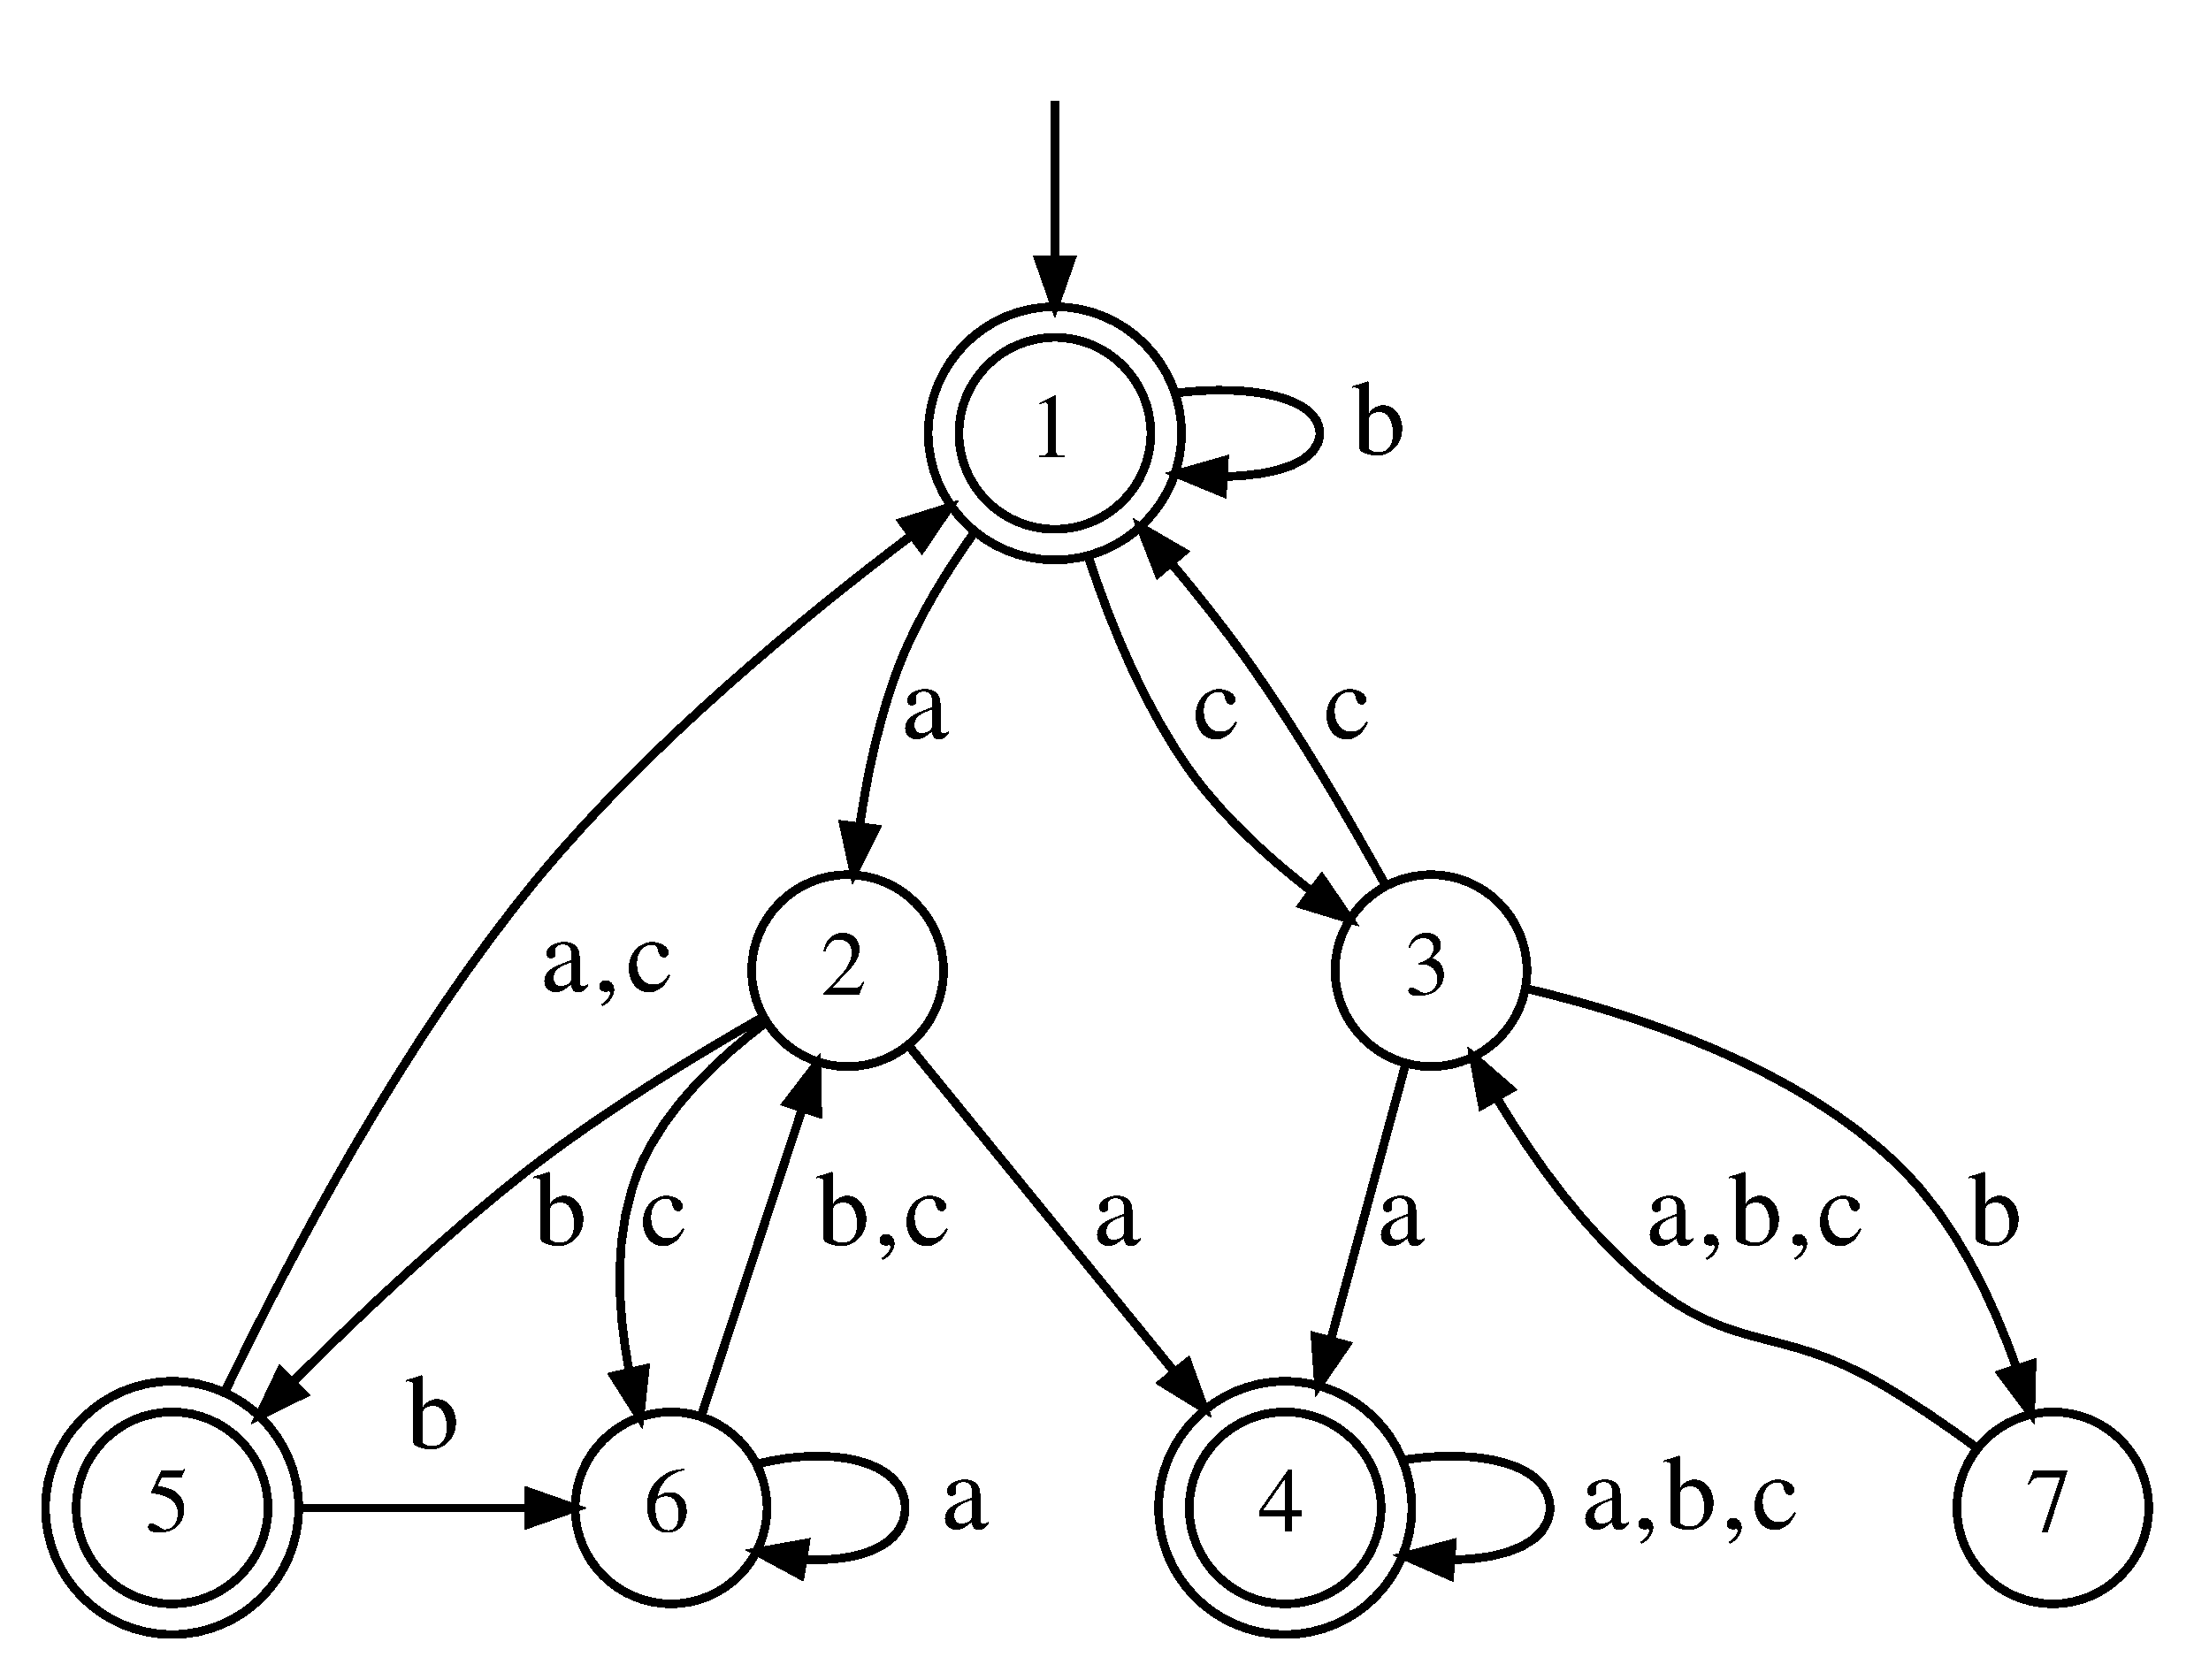
\includegraphics[scale=0.15]{img/datamod/BFS-example.eps}
    \else
      \input{img/BFS-example-a5}
    \fi
  }
  \hfill
  \subfloat[BFS traversal tree for the automaton shown in Figure~\ref{syn-en:img:bfs:bfs-ex}\label{syn-en:img:bfs:bfs-tree}]{
    \ifafour
      \input{img/BFS-tree-a4}
    % 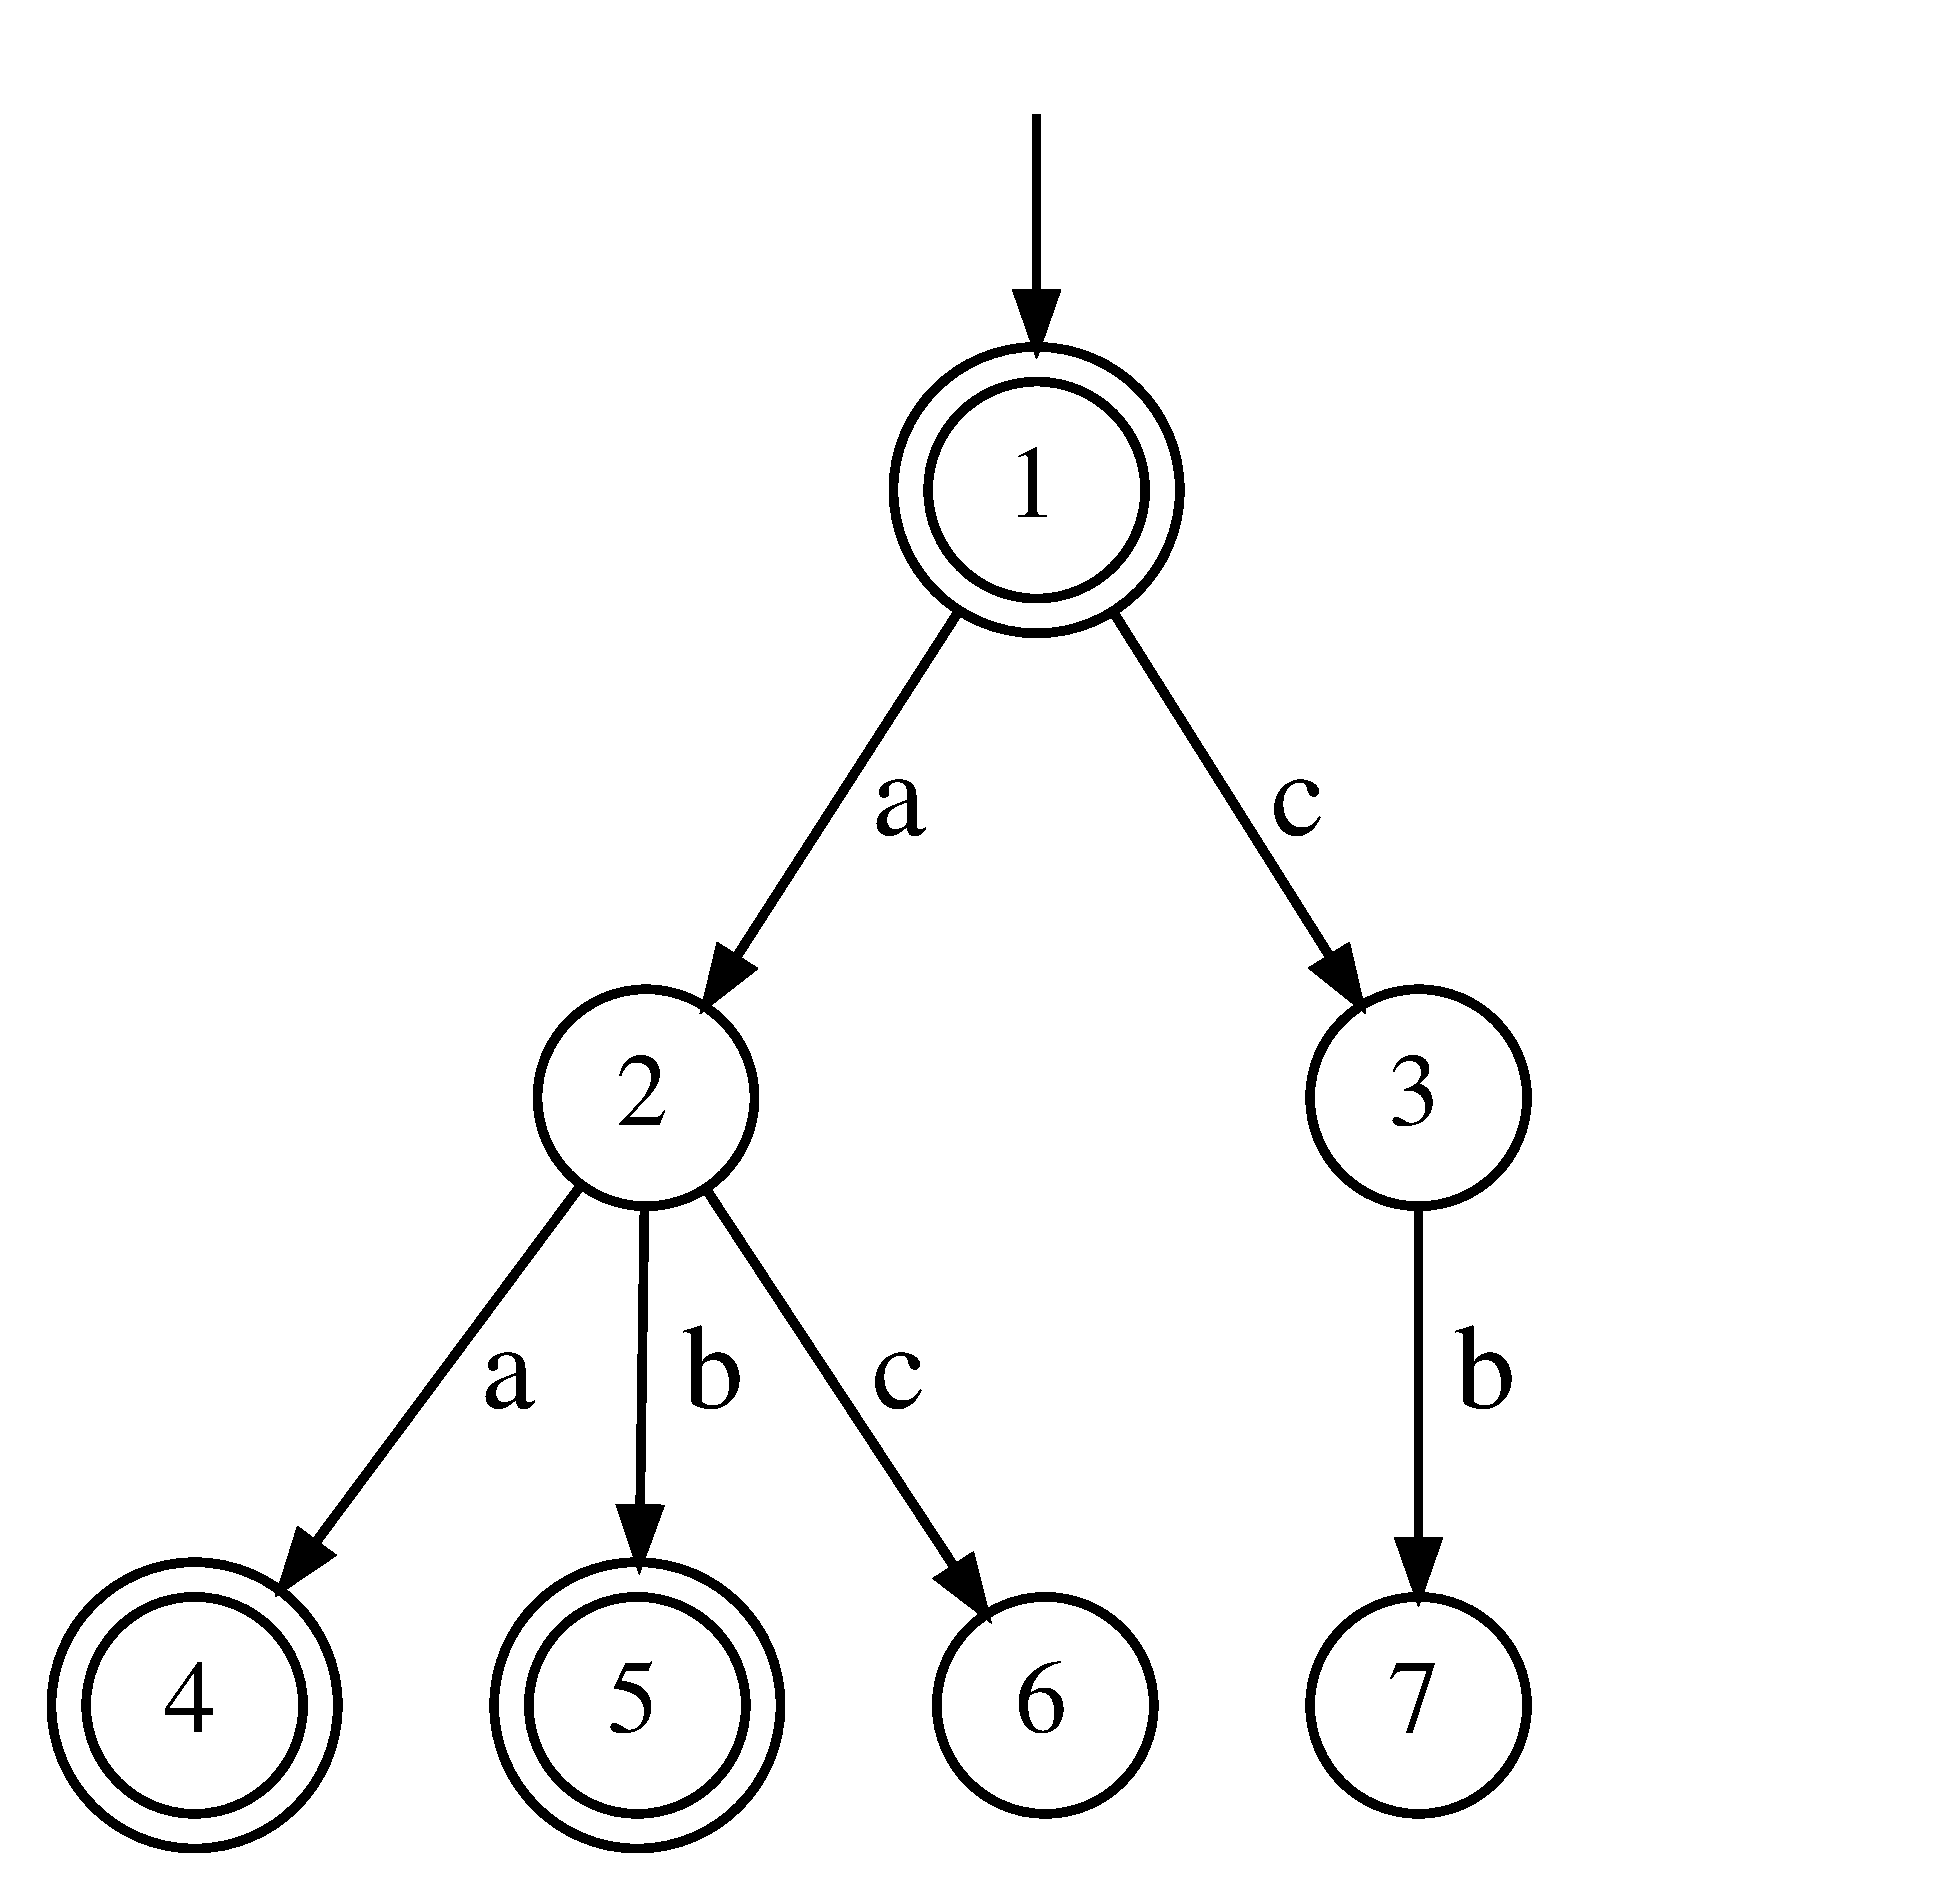
\includegraphics[scale=0.15]{img/datamod/BFS-tree.eps}
    \else
      \begin{tikzpicture}[
    ->, % makes the edges directed
    >=stealth', % makes the arrow heads bold
    node distance=1.7cm, % specifies the minimum distance between two nodes. Change if necessary.
    every state/.style={thick, fill=gray!10, minimum size = 0pt}, % sets the properties for each ’state’ node
    initial text=$ $, % sets the text that appears on the start arrow
]
    \def\xshift{0.53cm}

    \node[state, initial above, accepting] (q1) {$1$};
    \node[state] (q2) [below left of=q1] {$2$};
    \node[state] (q3) [below right of=q1] {$3$};
    \node[state, accepting] (q5) [below of=q2]  {$5$};
    \node[state, accepting] (q4) [left of=q5, xshift=\xshift]  {$4$};
    \node[state] (q6) [right of=q5, xshift=-\xshift]  {$6$};
    \node[state] (q7) [below of=q3]  {$7$};

    \path
        (q1) edge [left] node {a} (q2)
        (q1) edge [right] node {c} (q3)
        (q2) edge [left] node {a} (q4)
        (q2) edge [left] node {b} (q5)
        (q2) edge [right] node {c} (q6)
        (q3) edge [right] node {b} (q7)
        ;
\end{tikzpicture}
    \fi
  }
  \caption{An example of a BFS-enumerated automaton and the corresponding BFS traversal tree}
  \label{syn-en:img:bfs}
\end{figure}

\insectionen{\ref{sec:review:cegar}} the algorithm based on counterexample-guided abstraction refinement (CEGAR) is described.
Methods based on CEGAR are applicable in a situation when one needs to infer a model that corresponds to some given requirements, and a checking system (oracle) is available.
On the first step some model (possibly, random) is constructed.
Then, an iterative process of refining the current model is initiated: on each step the compliance of the current model to the requirements is checked using the oracle.
If the oracle check is successfully passed, then the sought model is found.
Otherwise, the oracle returns one or several counterexamples, which are consequently used to refine the model.

%------

\textbf{\underline{Chapter 2}} describes the development, implementation, and experimental evaluation of DFA inference methods with different approaches to reducing the 
search space during SAT solving.

\insectionen{\ref{sec:space:dfs}} a description of developed symmetry breaking predicates based on encoding the \emph{depth-first search}~(DFS) algorithm is provided.
The use of BFS-based symmetry breaking predicates has previously allowed increasing the efficiency of the \texttt{DFASAT} method considerably.
It was logical to consider as the next research task the development of symmetry breaking predicates based on the DFS algorithm and the method that uses them.
An example of a DFS-enumerated DFA is shown in Figure~\ref{syn-en:img:dfs:dfs-ex}, and~\ref{syn-en:img:dfs:dfs-tree} shows the corresponding traversal tree.

\begin{figure}[ht]
  \centering
  \subfloat[An example of a DFS-enumerated automaton\label{syn-en:img:dfs:dfs-ex}]{
    \ifafour
      % 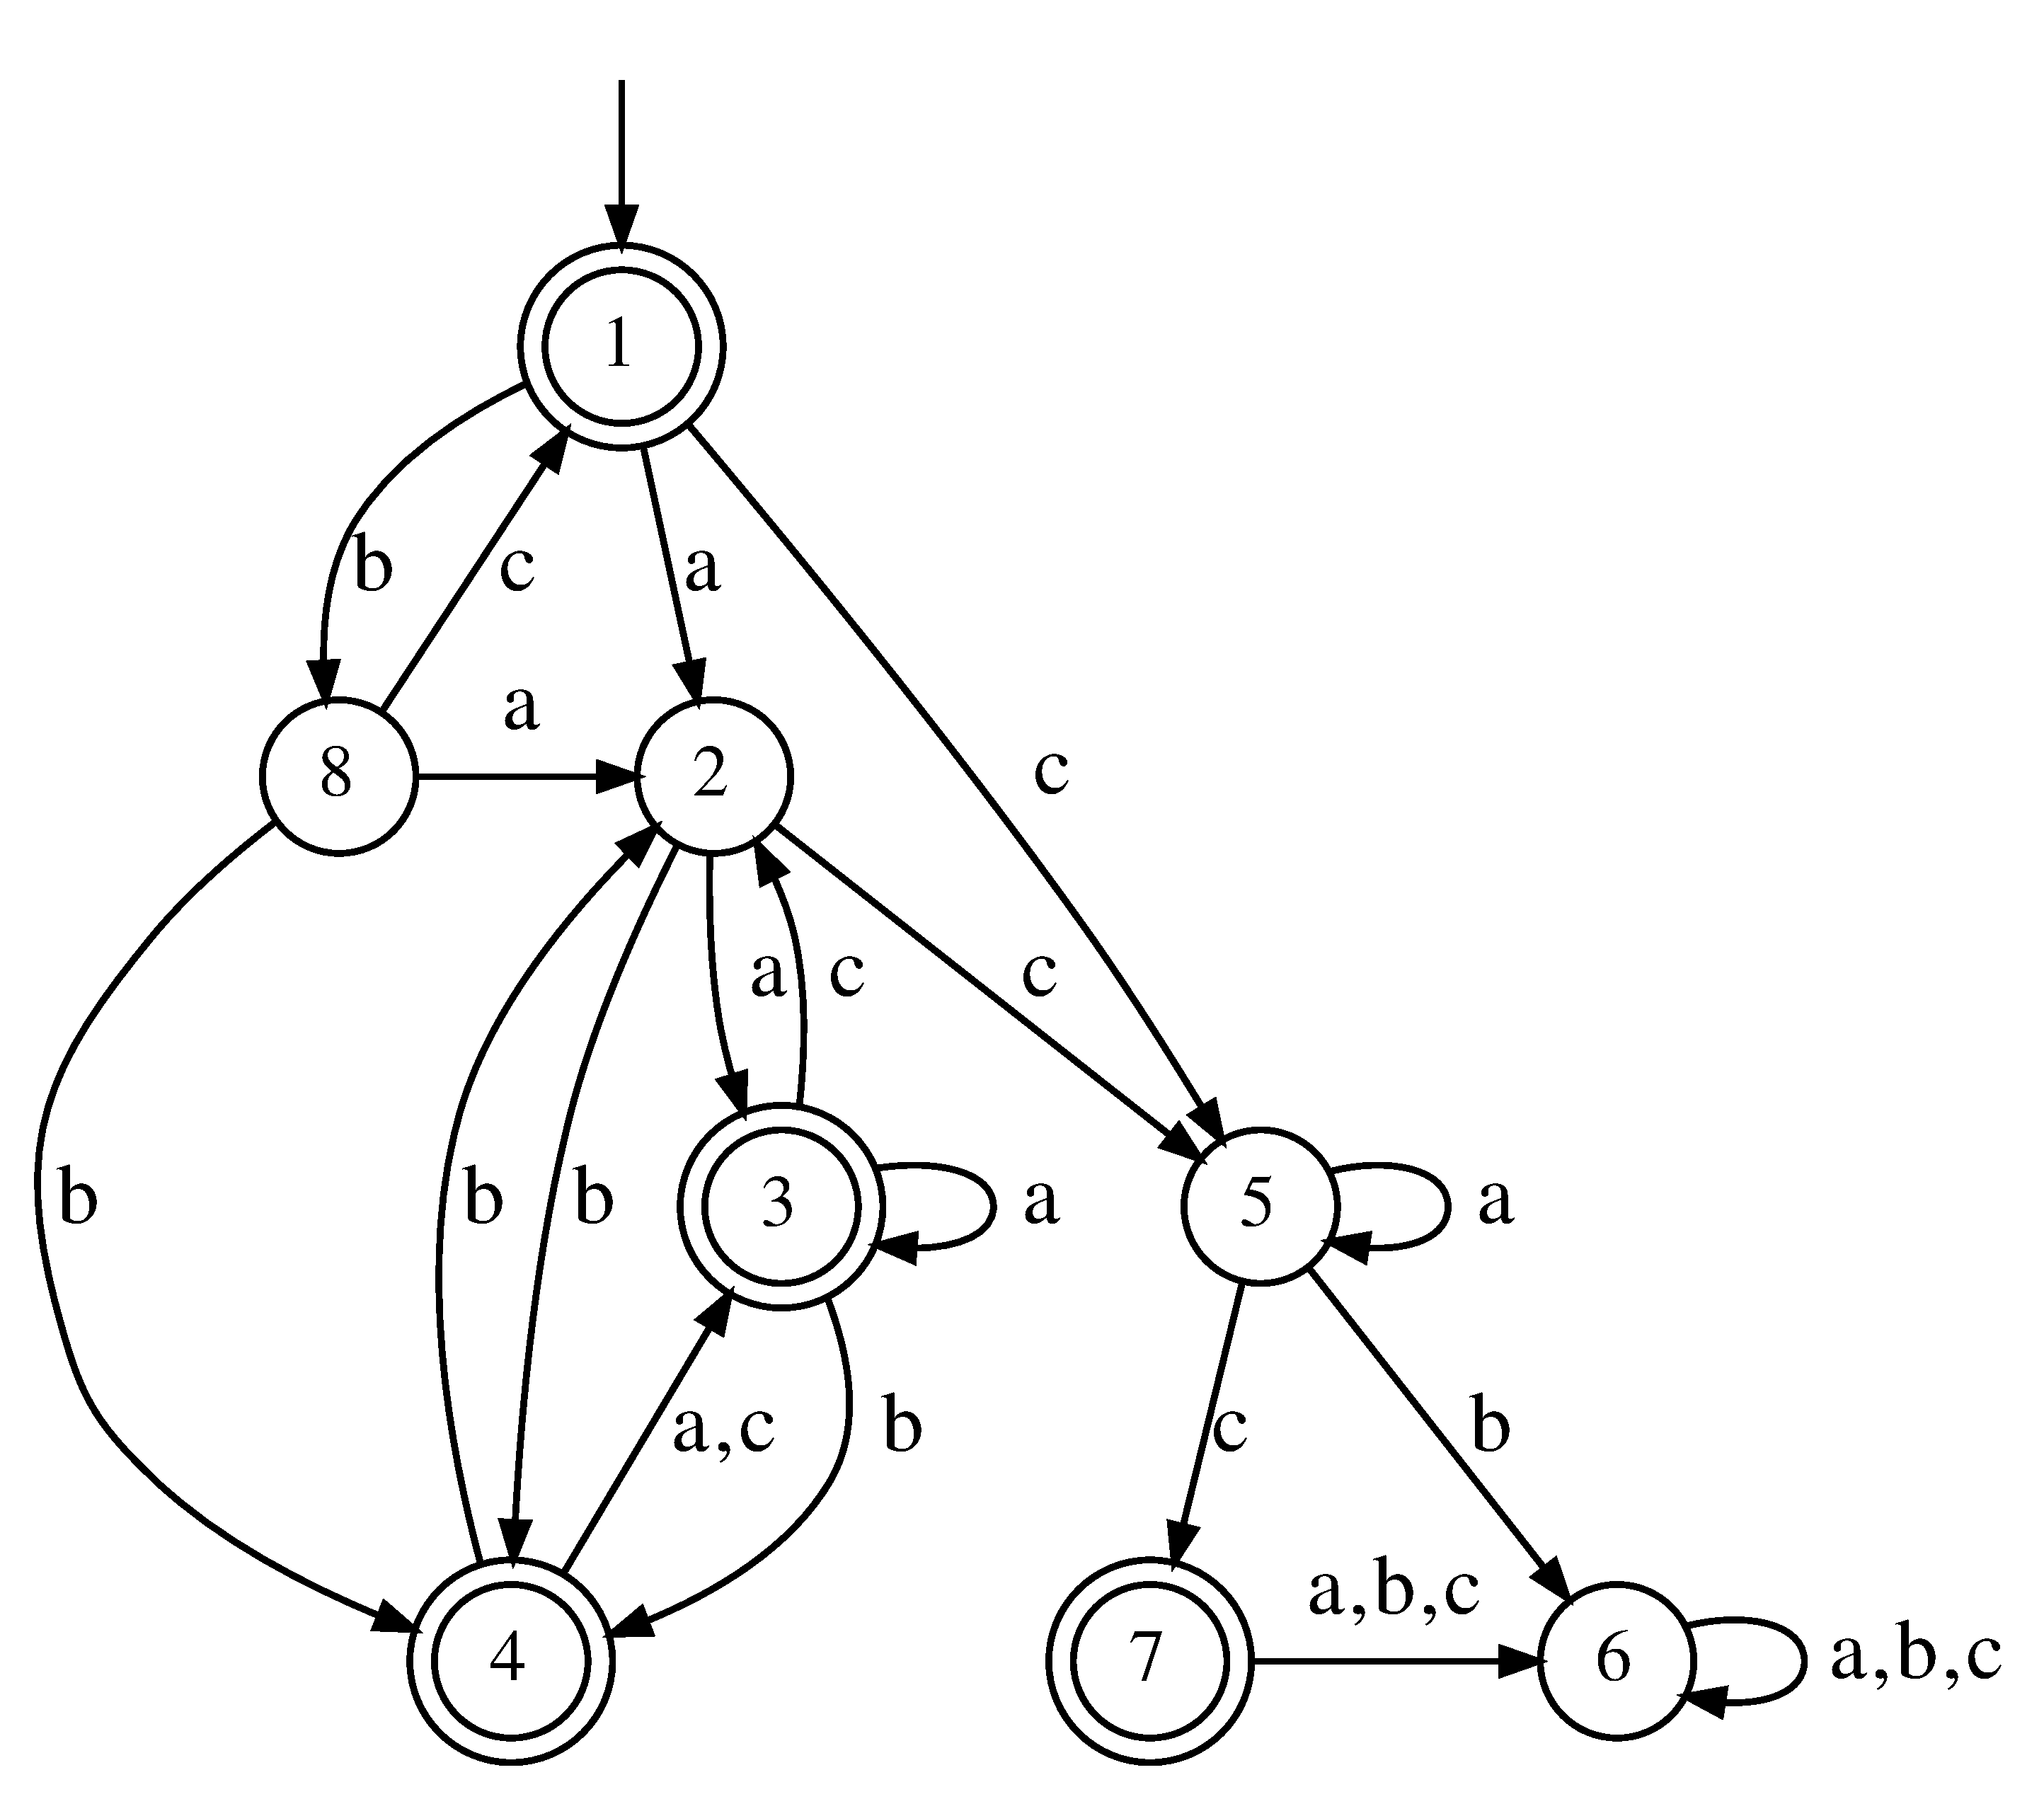
\includegraphics[scale=0.15]{img/datamod/DFS-example.eps}
      \input{img/DFS-example-a4}
    \else
      \begin{tikzpicture}[
    ->, % makes the edges directed
    >=stealth', % makes the arrow heads bold
    node distance=1.9cm, % specifies the minimum distance between two nodes. Change if necessary.
    every state/.style={thick, fill=gray!10, minimum size = 0pt}, % sets the properties for each ’state’ node
    initial text=$ $, % sets the text that appears on the start arrow
]
    \node[state, initial above, accepting] (q1) {$1$};
    \node[state] (q2) [below of=q1] {$2$};
    \node[state] (q8) [left of=q2] {$8$};
    \node[state] (q5) [right of=q2] {$5$};
    \node[state, accepting] (q4) [below of=q8] {$4$};
    \node[state, accepting] (q3) [below of=q2] {$3$};
    \node[state, accepting] (q7) [below of=q5] {$7$};
    \node[state] (q6) [right of=q7] {$6$};
    
    \path
        (q1) edge [bend right=10, left] node {b} (q8)
        (q8) edge [bend right=10, right] node {c} (q1)
        (q1) edge [right] node {a} (q2)
        (q1) edge [right] node {c} (q5)
        (q8) edge [above] node {a} (q2)
        (q2) edge [above] node {c} (q5)
        (q3) edge [loop below] node {a} (q3)
        (q5) edge [loop above] node {a} (q5)
        (q6) edge [loop below] node {a,b,c} (q6)
        (q5) edge [right] node {c} (q7)
        (q5) edge [right] node {b} (q6)
        (q7) edge [below] node {a,b,c} (q6)
        (q8) edge [left] node {b} (q4)
        (q4) edge [bend right=10, below] node {a,c} (q3)
        (q3) edge [bend right=10, above] node {b} (q4)
        (q2) edge [bend right=10, left] node {a} (q3)
        (q3) edge [bend right=10, right] node {c} (q2)
        (q4) edge [bend right=10, below] node [xshift=2pt, yshift=2pt] {b} (q2)
        (q2) edge [bend right=10, above] node {b} (q4)
        ;

\end{tikzpicture}
    \fi
  }
  \hfill
  \subfloat[The DFS traversal tree for the automaton in Figure~\ref{syn-en:img:dfs:dfs-ex}\label{syn-en:img:dfs:dfs-tree}]{
    \ifafour
      % 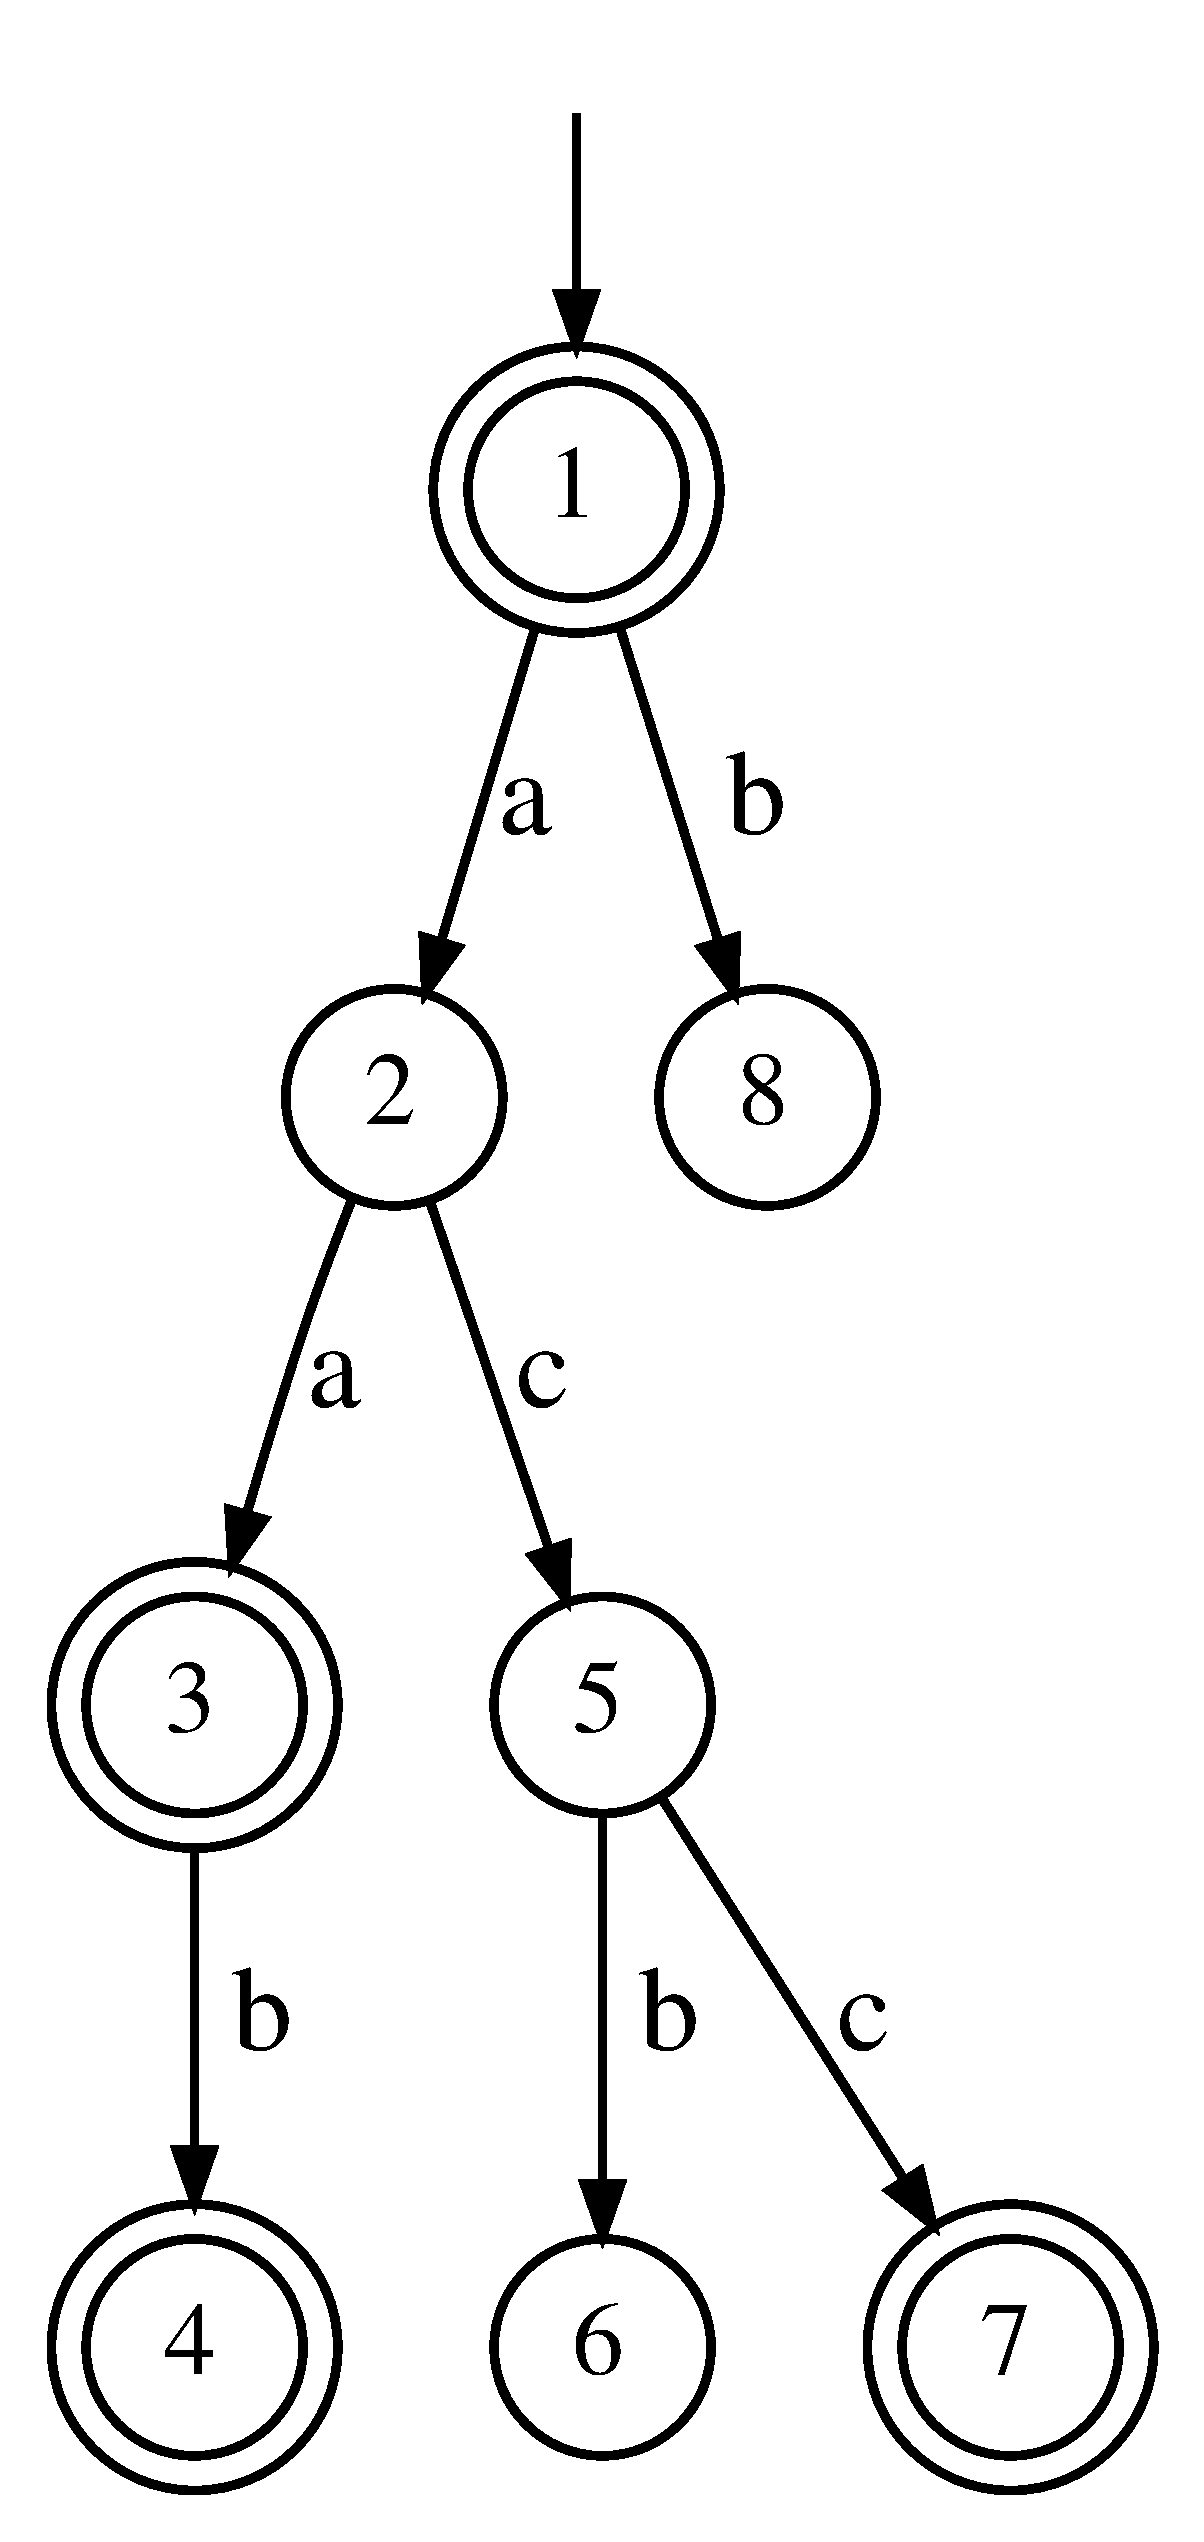
\includegraphics[scale=0.15]{img/datamod/DFS-tree.eps}
      \begin{tikzpicture}[
    ->, % makes the edges directed
    >=stealth', % makes the arrow heads bold
    node distance=2cm, % specifies the minimum distance between two nodes. Change if necessary.
    every state/.style={thick, fill=gray!10, minimum size = 0pt}, % sets the properties for each ’state’ node
    initial text=$ $, % sets the text that appears on the start arrow
    double distance between line centers=2pt
]
    \def\xshift{0.7cm}

    \node[state, initial above, accepting]     (q1)                 {$1$};
    \node[state] (q2) [below of=q1, xshift=-\xshift] {$2$};
    \node[state] (q8) [below of=q1, xshift=\xshift] {$8$};
    \node[state, accepting] (q3) [below of=q2, xshift=-\xshift] {$3$};
    \node[state] (q5) [below of=q2, xshift=\xshift] {$5$};
    \node[state, accepting] (q4) [below of=q3, xshift=-\xshift] {$4$};
    \node[state] (q6) [below of=q5, xshift=-\xshift] {$6$};
    \node[state, accepting] (q7) [below of=q5, xshift=\xshift] {$7$};

    \path
        (q1) edge [left] node {a} (q2)
        (q1) edge [right] node {b} (q8)
        (q2) edge [left] node {a} (q3)
        (q2) edge [right] node {c} (q5)
        (q3) edge [left] node {b} (q4)
        (q5) edge [left] node {b} (q6)
        (q5) edge [right] node {c} (q7)
        ;
\end{tikzpicture}
    \else
      \input{img/DFS-tree-a5}
    \fi
  }
  \caption{An example of a DFS-enumerated automaton and the corresponding DFS-traversal tree}
  \label{syn-en:img:dfs}
\end{figure}

The developed predicates are expressed as a CNF formula with $\mathcal{O}\left(M^{4} + M^{3} \times L^{2}\right)$ clauses, 
which is $M$ times greater than the number of clauses for the BFS-based DFA symmetry breaking predicates.

\insectionen{\ref{sec:space:tight}} a description of the developed compact BFS-based symmetry breaking predicates is given.

The compactness of the developed predicates consists in reduction of the size of the formula that encodes the BFS-based symmetry breaking predicates from
$\mathcal{O}\left(M^{3} + M^{2} \times L^{2}\right)$ to $\mathcal{O}\left(M^{2} \times L\right)$ clauses.
Analysis of constraints from the original encoding, which were expressed using $\mathcal{O}\left(M^{3}\right)$ и $\mathcal{O}\left(M^{2} \times L^{2}\right)$ clauses,
showed that some parameters that define the size of the formula are independent, and other parameters may be eliminated by introduction of new variables.
For each such constraint a way of making it more compact was developed, leading to an overall decrease of formula size.
Apart from this, the majority of clauses for the original encoding, which consisted of  $\mathcal{O}\left(M\right)$ literals,
were replaced by clauses comprised of two or three literals: this considerably influences the performance of SAT solvers, since such clauses are processed in constant time
and are not stored in memory~\cite{MSilva-SATbook09}.

\textbf{Section~\ref{sec:space:pruning}} describes developed search space reduction approaches for DFA inference, that are based on BFS tree structure properties, 
also on connections between the augmented prefix tree acceptor and the sought DFA.
Figure~\ref{syn-en:img:full-bfs} shows a complete BFS tree of an arbitrary size on an arbitrary $L$-sized alphabet.
The tree is called complete since each vertex has exactly $L$ children.

\begin{figure}[ht]
  \centering
  \scalebox{0.625}{%
\begin{tikzpicture}[scale=1.2, level 1/.style={sibling distance=60mm},level 2/.style={sibling distance=40mm}, level distance=25mm, level 3/.style={sibling distance=50mm}]
\node [ellipse,draw] (root){$1$}
  child {node [ellipse,draw] (a0) {$2$}
    child {node [ellipse,draw] (a0b0) {$L+2$}}
    child {node [ellipse,draw] (a0bj) {$L+j+1$}}
    child {node [ellipse,draw] (a0bL) {$2L+1$}}
  }
  child {node (aj) {$\vdots$}
    child {node [ellipse,draw] (r) {$r$}
      child {node [xshift=-0.25em,ellipse,draw] (r0) {$(r-1)L+2$}}
      child {node [ellipse,draw] (rj) {$(r-1)L+j+1$}}
      child {node [xshift=0.25em,ellipse,draw] (rL) {$rL+1$}}
    }
  }
  child {node [ellipse,draw] (aL) {$L+1$}
    child {node [ellipse,draw] (aLb0) {$L^2+2$}}
    child {node [ellipse,draw] (aLbj) {$L^2+j+1$}}
    child {node [ellipse,draw] (aLbL) {$L^2+L+1$}}
  }
;

\path (root) -- (a0) node [below, midway, darkblue] {$1$};
\path (root) -- (aL) node [below, midway, darkblue] {$L$};

\path (a0) -- (a0b0) node [below, midway, darkblue] {$1$};
\path (a0) -- (a0bj) node [left, midway, darkblue] {$j$};
\path (a0) -- (a0bL) node [below, midway, darkblue] {$L$};

\path (aL) -- (aLb0) node [below, midway, darkblue] {$1$};
\path (aL) -- (aLbj) node [left, midway, darkblue] {$j$};
\path (aL) -- (aLbL) node [below, midway, darkblue] {$L$};

\path (r) -- (r0) node [below, midway, darkblue] {$1$};
\path (r) -- (rj) node [left, midway, darkblue] {$j$};
\path (r) -- (rL) node [below, midway, darkblue] {$L$};

\path (a0) -- (aj) node [midway] {$..$};
\path (aj) -- (aL) node [midway] {$..$};

\path (a0b0) -- (a0bj) node [midway] {$..$};
\path (a0bj) -- (a0bL) node [midway] {$..$};

\path (aLb0) -- (aLbj) node [midway] {$..$};
\path (aLbj) -- (aLbL) node [midway] {$..$};

\path (r0) -- (rj) node [midway] {$..$};
\path (rj) -- (rL) node [midway] {$..$};
\end{tikzpicture}
%
%
\begin{comment}
%
%
\begin{figure}
\centering
\begin{tikzpicture}[scale=0.75, level 1/.style={sibling distance=60mm},level 2/.style={sibling distance=40mm}, level distance=25mm, level 3/.style={sibling distance=50mm}]
\node [ellipse,draw] (root){$1$}
  child {node [ellipse,draw] (a0) {$2$}
   child {node [ellipse,draw] (a0b0) {$L+2$}}
   child {node [ellipse,draw] (a0bj) {$L+j+2$}}
   child {node [ellipse,draw] (a0bL) {$2L+1$}}
  }
  child {node (aj) {$\vdots$}
    child {node [ellipse,draw] (r) {$r$}
      child {node [ellipse,draw] (r0) {$(r-1)L+2$}}
      child {node [ellipse,draw] (rj) {$(r-1)L+j+2$}}
      child {node [ellipse,draw] (rL) {$rL+1$}
        child [grow=right,red] {node [red] (j) {$0\leq j < L$} edge from parent[draw=none]}
      }
    }
  }
  child {node [ellipse,draw] (aL) {$L+1$}
    child {node [ellipse,draw] (aLb0) {$L^2+2$}}
    child {node [ellipse,draw] (aLbj) {$L^2+j+2$}}
    child {node [ellipse,draw] (aLbL) {$L^2+L+1$}}
  }
;

\path (root) -- (a0) node [midway, red] {$0$};
\path (root) -- (aL) node [midway, red] {$L-1$};

\path (a0) -- (a0b0) node [midway, red] {$0$};
\path (a0) -- (a0bj) node [midway, red] {$j$};
\path (a0) -- (a0bL) node [midway, red] {$L-1$};

\path (aL) -- (aLb0) node [midway, red] {$0$};
\path (aL) -- (aLbj) node [midway, red] {$j$};
\path (aL) -- (aLbL) node [midway, red] {$L-1$};

\path (r) -- (r0) node [midway, red] {$0$};
\path (r) -- (rj) node [midway, red] {$j$};
\path (r) -- (rL) node [midway, red] {$L-1$};

\path (a0) -- (aj) node [midway] {$..$};
\path (aj) -- (aL) node [midway] {$..$};

\path (a0b0) -- (a0bj) node [midway] {$..$};
\path (a0bj) -- (a0bL) node [midway] {$..$};

\path (aLb0) -- (aLbj) node [midway] {$..$};
\path (aLbj) -- (aLbL) node [midway] {$..$};

\path (r0) -- (rj) node [midway] {$..$};
\path (rj) -- (rL) node [midway] {$..$};
\end{tikzpicture}
\caption{Worst case BFS tree with $0\leq j <L$}
\end{figure}
%
%
\end{comment}
}
  \caption{A complete BFS tree with $\abs{\Sigma}=L$}
  \label{syn-en:img:full-bfs}
\end{figure}

Following an analysis of this tree some properties and constraints that are characteristic for a BFS tree were formulated.
For example, it has been proved that for a vertex with index $r$ in the complete tree, its rightmost child has index $rL + 1$.
Furthermore, we proved that then $rL + 1$ is the upper bound for the index of vertex $r$ in an arbitrary BFS tree.
Then we can state that in an arbitrary BFS tree a vertex with index $n$ can only have children with indices from the range from $r + 1$ to $rL + 1$.
Introduction of these constraints allows reducing the number variables used in the encoding and thus reduce this size of the resulting formula.

By definition, in any BFS tree the children of any vertex $r$ have consecutive indices, and there are no more than $L$ children.
We analyzed the connection between vertices of the APTA vertices and the DFA states.
If the prefix tree contains a path of length $k$ from the root to some vertex $t_{i}$, and vertex $t_{i}$ corresponds to state $d_{j}$ of the sought automaton, then
the automaton must contain a path of length no more than $k$ from the initial state to state $d_{j}$.
A SAT encoding of these properties was developed.
Augmentation of the formula with corresponding constraints allows for additional reduction of the search space during SAT solving.

\textbf{Section{\ref{sec:space:results}}} describes the developed software tool \texttt{DFA-Inductor-py} for DFA inference, implementation of developed methods as parts of 
this software tool, and results of experimental evaluation of all developed methods.

In the process of preparing this thesis a software tool \texttt{DFA-Inductor-py}~\cite{dfa-inductor-py-en} for DFA inference from behavior examples has been developed using the 
\emph{Python} programming language.
The tool is comprised of various modules for solving the problem of DFA inference from behavior examples, the problem of DFA inference from an excessive set of 
behavior examples, and the problem of inferring all non-isomorphic DFA from given behavior examples~(these methods are described in the following chapters).
The tool implements different symmetry breaking predicates, including ones previously proposed by other authors, and the ones developed in this thesis.

The developed software tool was used to perform two series of experimental evaluations.
First we compared two methods for DFA inference from behavior examples that use symmetry breaking predicates based on BFS and DFS, correspondingly.
Since these two methods are based on the method \texttt{DFASAT}, in which symmetry breaking constraints are based on fixing the enumeration of some large clique in the consistency graph, we also added \texttt{DFASAT} to this experimental evaluation.

Publicly open tests (sets of behavior examples), for example, from \emph{Abbadingo One DFA Learning Competition}~\cite{DBLP:conf/icgi/LangPP98} and \emph{StaMinA Competition}~\cite{DBLP:journals/ese/WalkinshawLDBD13}, were developed for inexact algorithms which can generate automata with hundreds of states.
Exact methods, both existing and proposed in this thesis, are currently not capable of inferring DFA of such size; for this reason, tests for this experimental evaluation
were generated randomly.
Experimental results are shown in Table~\ref{syn-en:tab:DFS-results} and allow drawing the conclusion that the use of DFS-based symmetry breaking predicates is impractical,
since the method that uses them is significantly inferior to the method that uses BFS-predicates.
However, note that the method that uses DFS-predicates still considerably outperforms \texttt{DFASAT}.
Nevertheless, based on experimental results, it was decided not to continue the development of DFS-predicates and concentrate on improving predicates based on the 
breadth-first search algorithm.

\begin{table}[ht]
  \caption{Median execution time in seconds for methods of DFA inference from behavior examples: method based on BFS symmetry breaking predicates, based on DFS symmetry breaking predicates, and the \texttt{DFASAT} method. Each value was calculated as a result of 100 independent runs on 100 problems. The execution of the methods was limited to one hour ($\text{TL} = 3600\,\, \text{seconds}$)}
  \centering
  \scalebox{0.95}{
    \begin{tabular}{cccccc}
      M & DFS     & & BFS    & & \texttt{DFASAT}\\
      \hline
      10 & 20.9   & & 20.5   & & 23.3  \\
      12 & 40.4   & & 37.6   & & 240.3 \\
      14 & 82.2   & & 62.4   & & ---   \\
      16 & 205.1  & & 114.1  & & ---   \\
      18 & 601.7  & & 181.9  & & ---   \\
      20 & 2501.6 & & 293.7  & & ---   \\
      22 & ---    & & 453.3  & & ---   \\
      24 & ---    & & 625.1  & & ---   \\
      26 & ---    & & 925.8  & & ---   \\
      28 & ---    & & 1314.4 & & ---   \\
      30 & ---    & & 1635.5 & & ---   \\
    \end{tabular}
  }
  \label{syn-en:tab:DFS-results}
\end{table}

In the second experimental evaluation we compared methods that use the original BFS-predicates (\texttt{DFA-Inductor}) and the BFS-predicates proposed in this thesis (\texttt{DFA-Inductor-py}).
As before, we also considered \texttt{DFASAT} and used randomly generated tests.
Comparison results of all three methods are depicted in Figure~\ref{syn-en:img:plots:cactus} and show that within a fixed time budget \texttt{DFA-Inductor-py} can solve more instances of the problem of DFA inference from behavior examples than \texttt{DFA-Inductor}: in ten minutes the new method solved 731 solved problems against 678 for the old one.
Also note that \texttt{DFASAT} cannot compete with two other methods.

Figure~\ref{syn-en:img:plots:scatter} depicts a more detailed compaison of \texttt{DFA-Inductor} и \texttt{DFA-Inductor-py}: one may notice that the method proposed in this thesis
shows better results for the vast majority of instances.

\begin{figure}[ht]
  \centering
  \begin{subfigure}[b]{0.48\textwidth}
    \centering
    \includegraphics[width=\textwidth]{img/lata19/plots/cactus}
    \caption{Comparison of methods \texttt{DFA-Inductor}, \texttt{DFA-Inductor-py}, and \texttt{DFASAT}, showing the number of problem instances solved within a fixed time budget}
    \label{syn-en:img:plots:cactus}
  \end{subfigure}%
  \;\;
  \begin{subfigure}[b]{0.48\textwidth}
    \centering
    \includegraphics[width=\textwidth]{img/lata19/plots/scatter}
    \caption{Detailed comparison of methods \texttt{DFA-Inductor} and \texttt{DFA-Inductor-py}, showing their performance for each problem instance}
    \label{syn-en:img:plots:scatter}
  \end{subfigure}
  \caption{Comparison results of the method that uses the original BFS-predicates (\texttt{DFA-Inductor}), the method that uses new BFS-predicates (\texttt{DFA-Inductor-py}), and \texttt{DFASAT}}
  \label{syn-en:img:plots}
\end{figure}

%------

\textbf{\underline{Chapter 3}} describes the development, implementation, and experimental evaluation of the exact method for DFA inference from an excessive set of behavior
examples using a reduction to SAT and counterexample-guided abstraction refinement.

\insectionen{\ref{sec:cegar:motivation}} we provide the study of the limits of applicability of methods proposed in previous chapters in dependence on the size of the augmented
prefix tree acceptor.
The size of the Boolean formula that encodes the DFA inference problem depends linearly on the size of the prefix tree:
$\mathcal{O}\left(N \times M^{2}\right)$ clauses, where $N$ is the size of the prefix tree and $M$ is the size of the DFA.
The number of variables in the Boolean formula also linearly depends on the size of the prefix tree: $\mathcal{O}\left(N \times M + M^{2}\right)$ variables.
Thus, when the sought automaton is fixed, the size of the Boolean formula and the number of its variables may vary considerably depending on the number of behavior examples and
their length.
As the size of the prefix tree increases, the SAT solver has to use more and more resources to store the formula and handle it, and the number of variables also increases.
This leads to a situation when the same automaton may be constructed by a SAT solver in seconds from a small set of behavior examples, and may not be found in hours and days in 
the case of an excessive number of long behavior examples.

Since in the case of DFA the key information about each behavior example (whether this word is accepted by the DFA) is contained in the last vertex of a path in the APTA corresponding to this word, it is doubtful that anything can be done in the case of long behavior examples.
However, in the case of an excessive number of behavior examples we can take only a subset of them and infer the same automaton faster.
The issue is in the way the behavior examples are selected: it is possible to accidently eliminate the examples that are necessary to generate the DFA that is the answer to the original problem,
and thus end up with a completely different DFA.
The next section proposes a method that solves this problem: it iteratively enumerates meaningful behavior examples from the original set.

\textbf{Section~\ref{sec:cegar:cegar-algo}} describes the proposed exact method for DFA inference from an excessive set of behavior examples, that is based on a reduction 
to SAT and the CEGAR approach.
As noted before, counterexample-guided abstraction refinement is commonly used in active learning problems.
The considered problem of DFA inference is, on the contrary, a passive learning problem.
However, in this thesis a method is proposed that solves the problem of DFA inference from behavior examples using ideas of the CEGAR approach.

Similar to the classical CEGAR, the proposed approach iteratively refines the model, which in this thesis is a deterministic finite automaton.
The initial prefix tree does not contain any vertices, but is augmented on each step.
On each step it is proposed to try inferring a DFA of the current size for the current prefix tree using a reduction to SAT.
If such a DFA does not exist, then, as before, the size of the sought DFA is increased by one, and the search process is repeated.
And if such an automaton is found, its compliance with the remaining behavior examples is checked.
If the DFA complies with all behavior examples, then the problem is solved.
If not, then we select one or several counterexamples from the behavior examples which are not safisfied by the DFA, and use them to augment the prefix tree,
build a new Boolean formula, and continue the search.
The scheme of the proposed method is shown in Figure~\ref{syn-en:img:cegar-algo}.

\begin{figure}[ht]
  \centering
  \includegraphics[scale=0.85]{img/ntv/cegar-en.pdf}
  \caption{Scheme of the exact method for DFA inference from an excessive set of behavior examples based on a reduction to SAT and the CEGAR approach}
  \label{syn-en:img:cegar-algo}
\end{figure}

Note that restarting the SAT solver after each augmentation of the prefix tree is extremely inefficient, since when new clauses are added to the formula, 
the search space of SAT is only reduced, and thus, there is no fundamental need to start searching for a satisfying assignment from scratch.
Incremental SAT solvers may be used to cope with this: after some satisfying assignment is found they switch to a state in which they wait for new clauses to be supplied,
and continue the search with a new refined formula from the same place where the search was paused before.


\textbf{Section~\ref{sec:cegar:results}} presents a description of the implementation of the developed method as a part of the tool \texttt{DFA-Inductor-py}, 
as well as results of experimental evaluation of the developed method.
In experimental evaluation we again used random tests.
Results of experimental evaluation showed that when the size of behavior examples $S=\abs{S_{+}}+\abs{S_{-}}$ exceeds $200 \times M$,
the CEGAR-based method works at least two times faster than the method that uses all behavior examples at once.
Moreover, the benefit of using CEGAR increases with the growth of the number of behavior examples.

%------

In \textbf{\underline{Chapter 4}} the problem of inferring all non-isomorphic DFA from given behavior examples is formulated, and the development, implementation, and
experimental evaluation of two methods that solve this problem is described.

\textbf{Section~\ref{sec:findall:problem}} provides a formal statement of the problem of inferring all non-isomorphic DFA of minimal size that satisfy given behavior examples.
As shown before, a DFA of minimal size yields a maximally exact generalization of given data expressed with behavior examples.
However, in the case when the behavior examples do not describe the sought automaton to a satisfactory degree, several different and minimal non-isomorphic automata may exist.
In this case a rational solution may be to infer all such automata for further analysis.
Figure~\ref{syn-en:img:find-all} shows all non-isomorphic minimal-sized DFA inferred for given behavior examples.
%
\begin{figure}[ht]
  \centering
  \ifafour
    \input{img/find-all-ex-tikz-compact-a4}
  \else
    \input{img/find-all-ex-tikz-compact-a5}
  \fi
  \caption{All non-isomorphic DFA corresponding to sets of behavior examples $S_{+} = \left\{a, bb, aaaa\right\}$ and $S_{-}=\left\{aa, bab\right\}$}
  \label{syn-en:img:find-all}
\end{figure}

Previously no methods for inferring all distinct minimal-sized DFA from given behavior examples have been proposed.
Moreover, without the use of symmetry breaking predicates based on BFS or DFS, that allow consideration of only one automaton for each isomorphism equivalence class instead of a factorial number of automata, efficient SAT-based inference of all distinct DFA does not seem possible.

\textbf{Section~\ref{sec:findall:SAT-based}} describes the method for inferring all non-isomorphic DFA of minimal size that uses a reduction to SAT and symmetry breaking.
When symmetry breaking predicates based on BFS or DFS are used, only a BFS-enumerated (DFS-enumerated) automaton can be inferred thus, it is sufficient to block the inferred automaton and
exclude it (along with all automata isomorphic to it) from the search space.
Note that in order to construct a DFA from the satisfying assignment, we only need to use values of transition variables $y_{i,l,j}$ and accepting state variables $z_{i}$.
This means that it suffices to forbid only the current values of these variables.
Denote $\varphi\left(q\right)$ the value of variable $q$ in the found satisfying assignment $\varphi$, and define a set $\mathcal{Y} = \{y_{i,l,j} | i,j \in \left[M\right] \wedge l \in \Sigma \wedge \varphi\left(y_{i,l,j}\right) = 1\}$.
Then, a \emph{blocking clause} can be defined as follows:
\begin{equation*}
\bigwedge_{y \in \mathcal{Y}} \neg y \wedge \bigwedge_{i \in \left[M\right]}\neg \varphi\left(z_{i}\right).
\end{equation*}

As in the CEGAR-based method, the addition of a blocking clause only reduces the size of the search space, so we do not have to restart the SAT solver, and may use it in 
incremental mode.

One more important property of the proposed method is the validation of the fact that the inferred automaton is the only existing minimal-sized automaton that satisfies given
behavior examples.
The uniqueness of a DFA in this case suggests that the given data sufficiently describes the found automaton.

\textbf{Section~\ref{sec:findall:results}} describes the implementation of the developed methods as parts of the tool \texttt{DFA-Inductor-py} and experimental evaluation.
Since previously there were no known efficient methods for inferring all distinct DFA from given behavior examples, in order to have a baseline we developed an enumerative backtracking algorithm which searches for all distinct DFA for given behavior examples without the use of external software tools.

Experimental results are summarized in Table~\ref{syn-en:tab:find-all}.
Experiments were run for three different groups of instances of the problem of DFA inference from given behavior examples.
In these three groups we used a different ratio between the number of behavior examples and the size of the inferred DFA:
for the first group the ratio was  $S = 5 \times M$, for the second group $S = 10 \times M$, and the third group had $S = 25 \times M$.
The column ``$>$1'' shows the percentage of problem instances for which more than one non-isomorphic DFA exists.

\begin{table}
  \centering
  \caption{Median execution time for inferring all distinct DFA with the SAT-based method that restarts the SAT solver~(REST), the SAT-based method that uses an incremental SAT solver~(INC), and the enumerative backtracking algorithm~(BTR)}
  \scalebox{0.8}{
    \begin{tabular}{ccccccccccccccc}
      \hline
      \multirow{2}{*}{$M$} & \multicolumn{4}{c}{$S = 5 \times M$}  & ~ & \multicolumn{4}{c}{$S = 10 \times M$} & ~ & \multicolumn{4}{c}{$S = 25 \times M$}\\\cline{2-5}\cline{7-10}\cline{12-15}
         & $>$1& REST  & INC    & BTR            & & $>$1& REST  & INC  & BTR             & & $>$1& REST & INC  & BTR            \\\hline
      5  & 53  & 2.3   & 2.0   & 0.8            & & 40  & 3.6   & 3.3  & 1.3             & & 17  & 4.1  & 3.4  & 1.5           \\ 
      6  & 56  & 2.8   & 2.4   & 2.1            & & 31  & 4.7   & 3.9  & 1.7             & & 27  & 5.4  & 4.3  & 1.7           \\ 
      7  & 87  & 3.9   & 2.5   & 4.1            & & 27  & 3.7   & 3.0  & 3.1             & & 13  & 7.4  & 6.7  & 2.5          \\ 
      8  & 80  & 4.6   & 3.7   & 87.2           & & 34  & 7.0   & 6.5  & 41.7            & & 16  & 10.1  & 8.9 & 11.6 \\ 
      9  & 91  & 7.6   & 3.9   & 475.1          & & 50  & 7.7   & 6.4  & 121.6           & & 10  & 13.8 & 13.0 & 61.4 \\ 
      10 & 89  & 15.7  & 5.3   & 2756.2         & & 47  & 8.6   & 7.0  & 974.7           & & 11  & 18.8 & 16.1 & 276.8 \\
      11 & 94  & 19.9  & 7.3   & ---            & & 63  & 18.5  & 13.8 & 3108.0          & & 9   & 24.5 & 21.9 & 1158.4 \\
      12 & 90  & 28.0  & 9.9   & ---            & & 49  & 22.3  & 16.7 & ---             & & 8   & 33.5 & 27.2 & 3289.1 \\
      13 & 92  & 185.5 & 18.1  & ---            & & 57  & 36.9  & 22.6 & ---             & & 12  & 62.0 & 51.4 & ---\\
      14 & 87  & 408.5 & 49.0  & ---            & & 71  & 85.1  & 41.8 & ---             & & 4   & 67.0 & 56.2 & ---\\
      15 & 95  & 571.1 & 174.1 & ---            & & 69  & 193.3 & 95.7 & ---             & & 6   & 29.2 & 26.2 & ---\\
      \hline
    \end{tabular}
  }
  \label{syn-en:tab:find-all}
\end{table}

Experimental results from Table~\ref{syn-en:tab:find-all} allow making the following conclusions:
\begin{enumerate}
  \item a first successful solution for the problem of inferring all distinct minimal-sized DFA from given behavior examples has been proposed;
  \item both SAT-based methods greatly outperfrom the backtracking method;
  \item as expected, the use of an incremental SAT solver gives a considerable advantage over the approach in which the solver is restarted: this is because after some DFA is found the intermediate state is preserved by the incremental SAT solver;
  \item the more behavior examples  are given for inferring a DFA, the less often a situation occurs when there are several different DFA corresponding to them.
\end{enumerate}


To \textbf{conclude}, the results of this study are:

%!TEX root = ../dissertation.tex

\begin{enumerate}
  \item Symmetry breaking predicates based on SAT encodings of the breadth-first search and depth-first search algorithms for reducing the search space reduction during SAT solving, and exact methods for DFA inference from behavior examples 
  that use these predicates, have been developed.
  The symmetry breaking predicates based on the encoding of the depth-first search algorithm have a rather theoretical
  significance, since they have not demonstrated any advantage over predicates based on the breadth-first search 
  algorithm encoding.
  The encoding of the symmetry breaking predicates based on breadth-first search is expressed with an asymptotically 
  smaller number of clauses in comparison to the previously proposed encoding.
  The developed exact method that uses these predicates together with predicates based on characteristics of the BFS traversal tree demonstrates better performance in comparison to previous methods.

  \item A new exact method for DFA inference from an excessive set of behavior examples that uses a reduction to SAT and counterexample-guided abstraction refinement has been developed.
  The size of the Boolean formula and the number of used variables linearly increase with the growth of the number of 
  behavior examples.
  The developed method allows inferring a DFA from an excessive set of behavior examples by iteratively augmenting
  the set of used behavior examples, completing the augmented prefix tree and using the SAT solver in incremental mode. 
  Since the set of used behavior examples is augmented with counterexamples to inferred intermediate DFA, as a result only 
  meaningful behavior examples are used for inference.
  Thus, this method allows for an exact solution of problems which previously could not be solved due to a large size of the Boolean formula.
  
  \item A method for inferring all non-isomorphic DFA of minimal size satisfying given behavior examples has been developed that uses symmetry breaking predicates and SAT solvers.
  Previously, the problem of inferring all minimal non-isomorphic DFA did not have an efficient solution, since
  isomorphic automata, being equivalent in structure and defined language, are deemed to be distinct by a SAT solver, leading to considering $\mathcal{O}\left(M!\right)$ isomorphic automata with $M$ states.
  The use of symmetry breaking predicates based on an encoding of the breadth-first search algorithm allows the SAT solver to consider only one representative of each isomorphism equivalence class instead of a factorial number of automata.
  Thus, a method for solving the problem of inferring all minimal-sized non-isomorphic DFA has been first proposed.
  The search for all non-isomorphic automata may be useful for their further analysis, and also for analysis of existing behavior examples.
  Another application of the developed method is the possibility to prove the uniqueness of the minimal automaton that 
  satisfies given behavior examples.
  
  \item During thesis preparation an open source software tool \texttt{DFA-Inductor-py} has been developed in \emph{Python} for the purpose of DFA inference from given behavior examples.
  The software tool is comprised of different modules for solving the problem of DFA inference from given behavior examples, the problem of inferring a DFA from an excessive set of behavior examples, and the problem of inferring all non-isomorphic DFA from given behavior examples.
  The tool implements different symmetry breaking predicates, including the ones developed by other authors and the ones developed in this thesis.

  \item The results of this thesis were used in the educational process of the Faculty of Information Technologies and Programming in the course ``Design of automata-based programs'' of the Bachelors's program ``Mathematical models and algorithms in software engineering'' (supported by the official act of use).

  \item A part of results have been used in the project SAUNA (``Integrated safety assessment and justification of nuclear power plant automaton'') by the ``IT in Industrial Automation'' research group of the department of electrical engineering and automation in Aalto University, Finland, in the framework of the Finnish research program in safety of nuclear power plants SAFIR2018.  This is confirmed by a letter from the principal investigator of the “IT in Industrial Automation” group, Valeriy Vyatkin.

  \item Results of this thesis have also been used in the project No.~18-37-00425 ``Development of efficient machine learning methods for deterministic finite automata inference based on Boolean satisfiability solving'' (2018--2020) funded by the Russian Foundation for Basic Research and led by the author of the thesis, and in research projects in the framework of the Russian academic excellence project <<5-100>>.
\end{enumerate}


The exact method for DFA inference from given behavior examples that uses symmetry breaking predicates based on 
the breadth-first first algorithm demonstrates better performance the previously known methods and allows inferring
larger automata in less time.
The method for inferring a DFA from an excessive set of behavior examples allows inferring automata from data, for which
the previously known methods could not infer any DFA in principle due to a large size of the Boolean formula.
The method for inferring all minimal-sized non-isomorphic DFA satisfying given behavior examples is the first known
method that allows inferring all non-isomorphic DFA: previously known methods may adapted to finding all DFA, 
but their application leads to a combinatorial explosion of the size of considered DFA due to lack of efficient 
symmetry breaking predicates.
The aim of this thesis was to increase the efficiency of exact methods for DFA inference from given behavior examples by reducing the search space during Boolean satisfiability problem solving.
Thus, according to experimental results, the aim is achieved.


\paragraph*{Acknowledgement.}
The author expresses gratitude to his supervisor, V.~Ulyantsev, Ph.D., for invaluable assistance in research and in preparation of this thesis, Prof.~A.~Shalyto for mentoring, colleagues from the International Laboratory ``Computer Technologies'', D.~Chivilikhin, Ph.D., for numerous consultations on research and for help with the English translation of the synopsis, K.~Chukharev and D.~Suvorov for help in preparing illustrative material for this thesis, A.~Bugrovsky and T.~Galimzhanov for their help with documents for preparing the defense of this thesis, and to foreign colleagues A.~Ignatiev, Ph.D., and Prof.~J.~Marques-Silva, Dr.~habil., for organizing and active participation in the internship, within the framework of which part of the author's research was carried out.

The author is also grateful to his parents, Timur and Valentina, for the fostered love of knowledge and mathematics, to Lazareva Ekaterina for always being there, to his friends Alexander B., Alexander S., Anastasia, Valentin, Eugene, Marina, Matvey, Natalya, Talgat and Tatiana for the moral support provided.